%
% robertson.tex -- Robertson Walker Metrik
%
% (c) 2017 Prof Dr Andreas Müller, Hochschule Rapperswil
%
\chapter{Kosmologie%
\label{skript:chapter:kosmologie}}
\lhead{Kosmologie}
\rhead{}
Die Einstein-Gleichungen ermöglichen erstmals, die Entwicklung
des ganzen Universums zu modellieren.
Dazu sind allerdings die Kenntnis der grossräumigen
Masseverteilung notwendig.
Es stellt sich heraus, dass diese im grossen isotrop und homogen ist.
Dies bedeutet, dass auch die Krümmung im Universum homogen und isotrop
ist.
Die Robertson-Walker-Metrik erfüllt diese Voraussetzung.
\index{Robertson-Walker-Metrik}%

\section{Massenverteilung im Universum}
\rhead{Massenverteilung im Universum}
Lange Zeit galt die Erde als das Zentrum des Universums.
Nikolaus Kopernikus hat mit dem heliozentrischen Modell der Erde
\index{Kopernikus, Nikolaus}%
diese privilegierte Stellung genommen.
Wilhelm Herschel war der erste Astronom, der sich darüber Gedanken
gemacht hat, wo innerhalb unserer Milchstrasse unser Sonnensystem
einzuordnen wäre.
Heute wissen wir, dass die Erde eher am Rande der Milchstrasse liegt.
Doch auch die Milchstrasse ist nichts besonderes, sie ist eine eher
unterdurchschnittliche Galaxie in einem durchschnittlichen
Galaxienhaufen.
Man kann diese Beobachtungen zusammenfassen im sogenannten
{\em kosmologischen Prinzip}, welches besagt, dass an unserem
\index{kosmologisches Prinzip}%
Standort im Universum nichts speziell ist.

Aus dem kosmologischen Prinzip lassens ich zwei Voraussetzungen
ableiten, denen ein kosmologisches Modell genügen muss, nämlich
Homogenität und Isotropie.
Die nächsten beiden Abschnitte klären deren Bedeutung und untermauern
sie mit Beobachtungsdaten.

\subsection{Isotropie}
\index{Isotropie}%
Isotropie bedeutet, dass es im Universum keine bevorzugte Richtung
gibt.
Auf kurze Distanzen stimmt dies ganz offensichtlich nicht.
In einer Kugel von wenigen Metern Durchmesser um den Beobachter
gibt es eine objektiv bevorzugte Richtung, die Richtung des Schwerfeldes
der Erde zum Erdmittelpunkt.
Aber auch in einer Kugel von etwa einer Milliarde Kilometer um
den Beobachter gibt es eine bevorzugte Richtung, nämlich die
Richtung zum hellsten und massivsten Stern, der Sonne.
Selbst in einer Kugel von etwa 3~Mpc\footnote{Mpc = 1 Million parsec,
ein parsec entspricht
$30.857\cdot 10^{16}\,\text{m} = 3.26\,\text{Lichtjahren}$.}
kann man eine bevorzugte Richtung finden, nämlich die Richtung zur grössten
und hellsten Galaxie des lokalen Haufens, der Andromeda-Galaxie M31.
\index{Andromeda-Galaxie}%
Erst in einer Kugel mit einem Radius von etwa 100Mpc gibt es keine
bevorzugte Richtung mehr. 

\begin{figure}
\centering
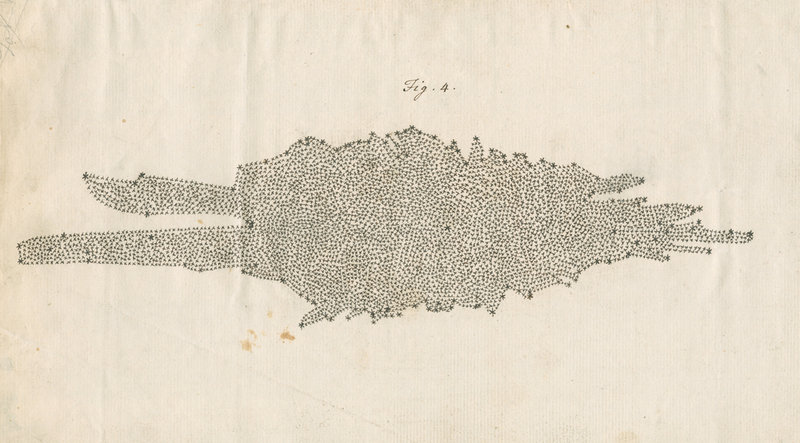
\includegraphics[width=\hsize]{chapters/images/rs-9810.jpg}
\caption{Karte der Milchstrasse von Willhelm Herschel aus dem Jahr 1785.
\label{skript:robertson:herschel}}
\end{figure}
Den erste Versuch, die Isotropie des Universums experimentell zu untersuchen,
hat Willhelm Herschel 1785 unternommen.
Herschel hat die Sterndichte in jede Richtung in der Ebene der Milchstrasse
ausgezählt.
Unter den (falschen) Annahmen, dass die Dichte innerhalb der Milchstrasse
konstant ist und man in alle Richtungen gleich weit und alle Sterne sehen
kann, kam er zu der Karte der Milchstrasse in
Abbildung~\ref{skript:robertson:herschel}.
Offenbar ist die sichtbare Milchstrasse auch in der Ebene der Milchstrasse
nicht isotrop.
Dies hat einerseits mit der Tatsache zu tun, dass sich die Sonne etwa
$26\,000$ Lichtjahre vom Zentrum der Galaxie entfernt befindet, andererseits
verdecken Staubwolken den Blick auf grosse Gebiet in der galaktischen Ebene.
Solche statistische Methoden müssen also auf wesentlich grössere Teile
des Universums angewendet werden.

Die Isotropie des Universums kann experimentell verifiziert werden,
indem man in alle Richtungen Galaxien zählt.
Weit entfernte Galaxien sollte es in jeder Richtung ungefähr mit 
gleicher Dichte geben.
Man beachte, dass es für diese Beurteilung nicht nötig ist, die
Distanz der Galaxien zu kennen, denn für Isotropie kommt es nur
auf die Richtung an.

\begin{figure}
\centering
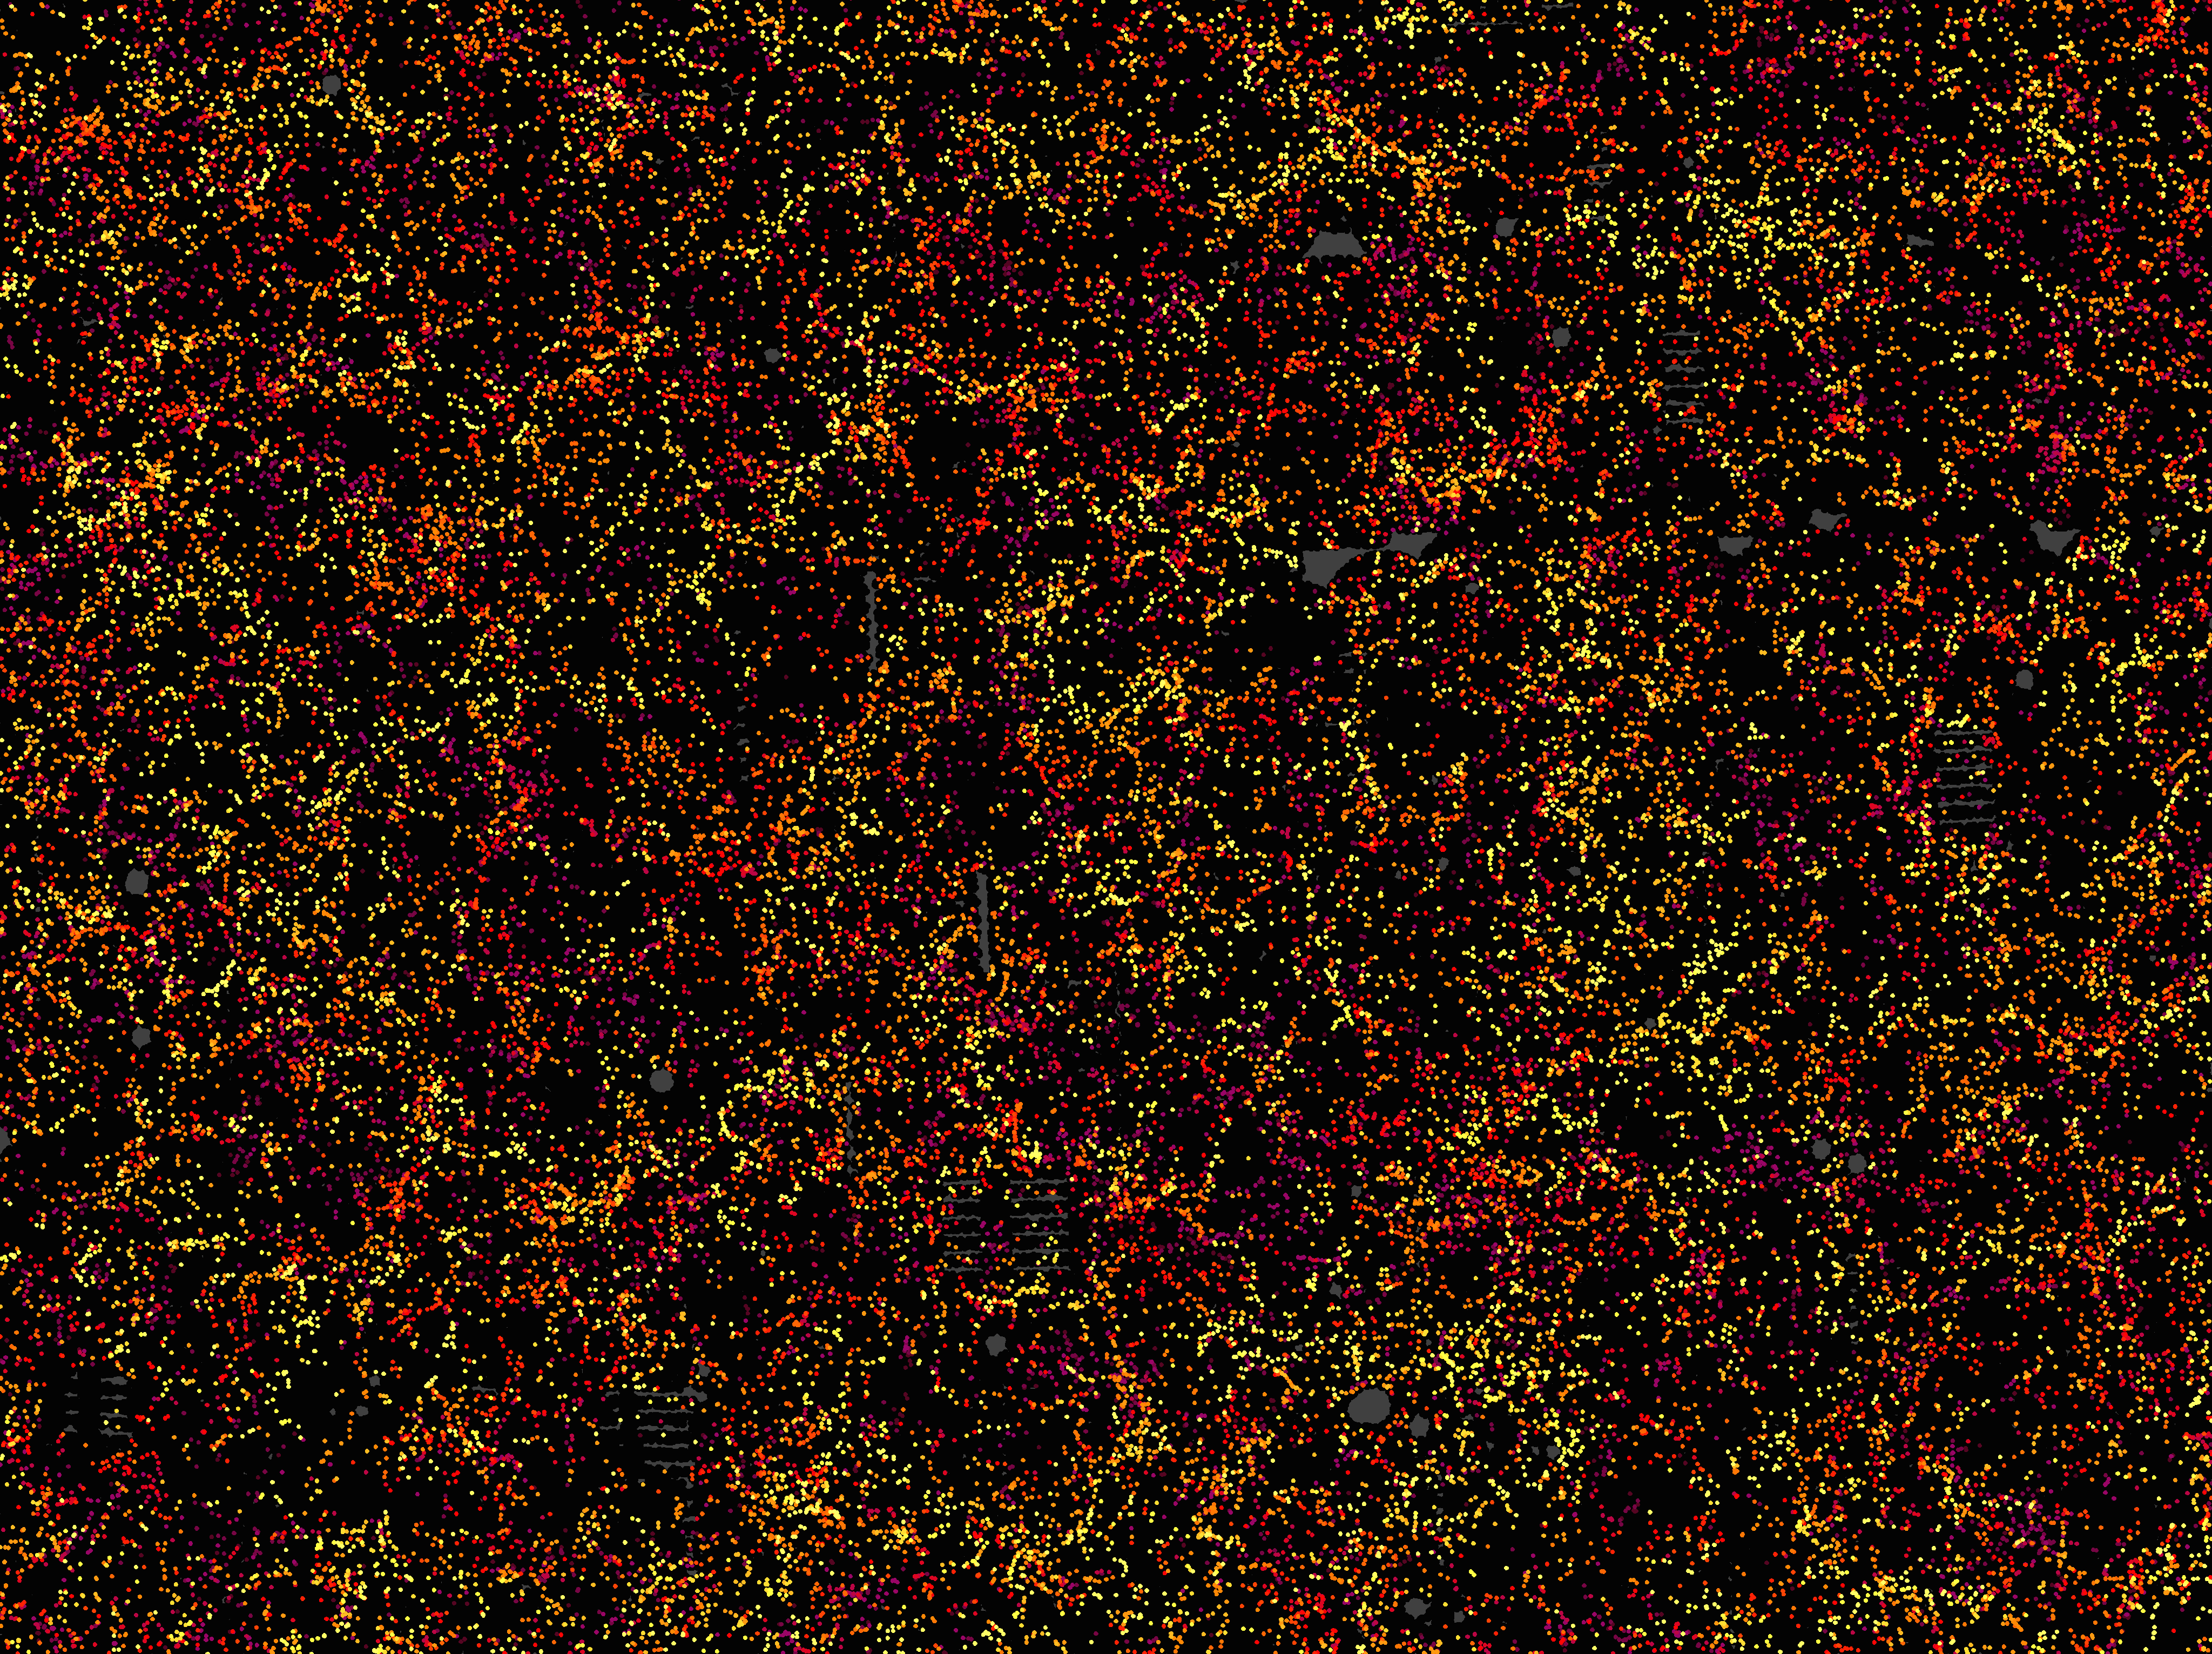
\includegraphics[width=\hsize]{chapters/images/cmass.png}
\caption{Verteilung von $48\,741$ Galaxien aus der Sloan Digital
Sky Survey \cite{skript:cmass} über einen Ausschnit von etwa
$1/20$ des Himmels.
Es sind zwar deutliche Zusammenklumpungen zu sehen, jenseits der
typischen Grösse dieser Cluster und Supercluster von Galaxien
ist die Verteilung im Mittel ziemlich gleichmässig.
\label{skript:robertson:cmass}}
\end{figure}

Die Sloan Digital Sky Survey \cite{skript:sdss} hat über mehrere
\index{Sloan Digital Sky Survey}%
Jahre vom Apache Point Observatorium aus über 1.2 Millionen Galaxien
vermessen.
Die Abbildung~\ref{skript:robertson:cmass} zeigt $48\,741$ Galaxien in
einem Auschnitt von etwa 1/20 des Himmels.
Es ist erkennbar, dass Galaxien sich zu Clustern und Superclustern
zusammenklumpen, aber jenseits deren typischen Abmessungen ist die
Verteilung ziemlich gleichmässig.
Die Sloan Digital Sky Survey scheint also auf den ersten Blick
die Hypothese der Isotropie zu bestätigen.
Eine zuverlässigere Aussage würde jedoch erfordern, die Galaxienverteilung
statistisch zu untersuchen.

\subsection{Homogenität}
\begin{figure}
\centering
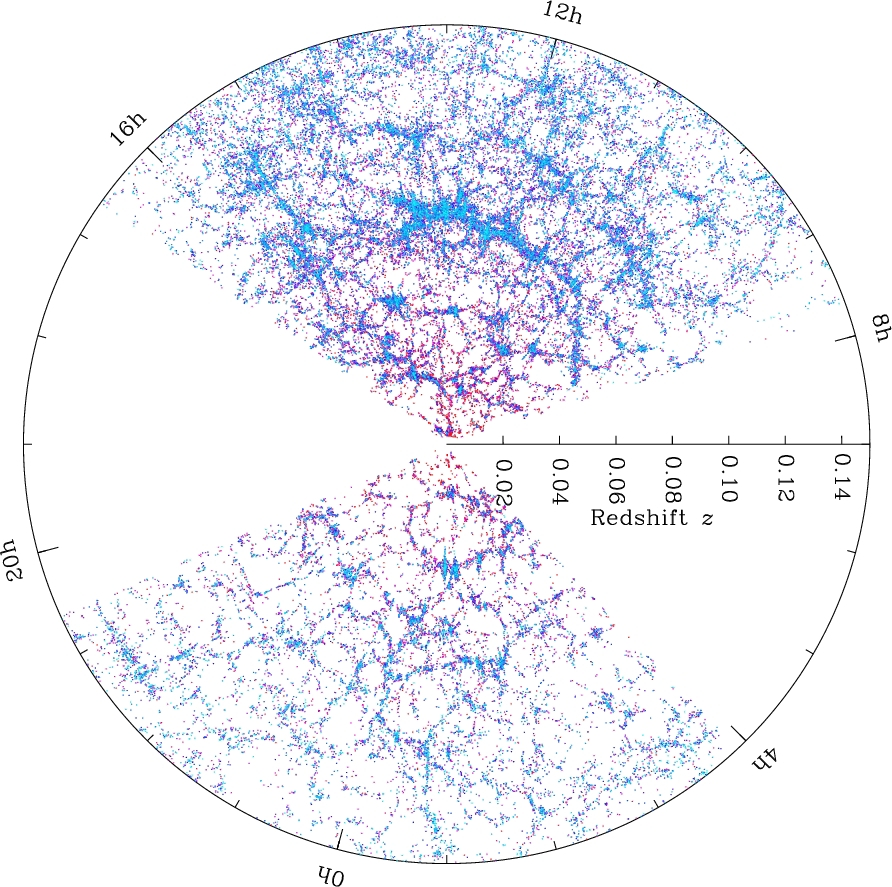
\includegraphics[width=\hsize]{chapters/images/orangepie-negative.jpg}
\caption{Verteilung der Galaxiender Sloan Digital Sky Survey.
Die beiden leeren Sektoren stellen Bereiche dar, in denen unsere
Milchstrasse zuverlässige Beobachtungen verunmöglicht.
Jeder Punkt stellt eine Galaxie dar.
\label{skript:robertson:orangepie}}
\end{figure}
\index{Homogenität}%
Homogenität bedeutet, dass es keinen bevorzugten Standort im Universum gibt.
Auf kurze Distanzen gilt dies ganz offensichtlich nicht.
In einer Kugel von einigen tausend Kilometern um den Beobachter ist
die Erde als massivstes Objekt ein bevorzugter Standort.
In einer Kugel von einer Milliarde Kilometer um den Beobachter ist
die Sonne als massivstes hellstes Objekt bevorzugt.
In einer Kugel von $100\,000$ Lichtjahren um den Beobachter ist das Zentrum
der Milchstrasse mit dem dortigen supermassiven schwarzen Loch ein
bevorzugter Ort.
In einer Kugel von etwa 3~Mpc ist der Schwerpunkt des lokalen Galaxienhaufens
ein bevorzugter Ort.
Bei grösseren Radien findet man zwar noch Cluster von Galaxien und
Supercluster, also Cluster von Galaxienclustern, aber jenseits von
etwa 100 Mpc scheint es keine noch grösseren Strukturen mehr zu geben.
In diesen Grössenordnungen kann man daher das Universum als homogen
bezeichnen.

Die Sloan Digital Sky Survey hat nicht nur die Richtungsverteilung von
Galaxien bestimmt, sondern auch deren Rotverschiebung.
Wie wir heute wissen, ist dies mindestens für ferne Galaxien ein ausreichend
genaues Mass für die Entfernung.
Abbildung~\ref{skript:robertson:orangepie} zeigt die Resultate.
Auch auf diesem Bild erkennt man wie schon in
Abbildung~\ref{skript:robertson:cmass}, dass Galaxien sich zu Clustern
und Filamenten gruppieren.
Dazwischen gibt es grosse leere Räume.
Jenseits der Dimensionen dieser Strukturen scheint die Verteilung jedoch
ziemlich gleichmässig zu sein.
Die Hypothese der Homogenität scheint also von den Beobachtungen der
Sloan Digital Sky Survey gestützt zu werden.
Eine zuverlässigere Aussage würde wieder eine statistische Anlyse der 
Daten erfordern.

\subsection{Energie-Impuls-Tensor}
Ein homogenes und isotropes Universum hat auch einen homogenen
und isotropen Energie-Impuls-Tensor.
Für ein ideales Gas wurde der Energie-Impuls-Tensor schon in
Abschnitt~\ref{skript:speziell:subsection:idealesgas}
in Gleichung~\eqref{skript:speziell:idealesgas} angegeben, er ist
\[
T^{\mu\nu} = pg^{\mu\nu} + (p+\varepsilon)u^\mu u^\nu.
\]
Das Universum ist jedoch nicht nur mit Gas gefüllt, sondern auch
mit Staub und Strahlung und eventuell weiteren, nicht bekannten
Komponenten.
Unabhängig von der Art der Komponenten ist die Energiedichte
im heutigen Universum sehr gering, nämlich weniger als ein Wasserstoffatom
pro Kubikmeter.
Die Atome treffen äusserst selten aufeinander,
der Druck des idealen Gases ist also sehr gering.

Staub als Komponenten zeichnet sich zum Beispiel dadurch aus, dass die Körner
jeweils aus einer grossen Zahl von Atomen zusammengesetzt sind.
Bei gleicher Dichte sind also Staubkörner noch seltener und damit kommen
Stösse praktsich nicht mehr vor.
Staub hat daher keinen Druck, der Energie-Impuls-Tensor vereinfacht sich zu
\[
T^{\mu\nu}
=
\varepsilon u^\mu u^\nu.
\]

Die im Universum enthaltene Strahlung muss ebenfalls in den
Energie-Impuls-Tensor einfliessen.
Es liegt nahe, sie wie ein
ideales Gas zu modellieren, doch das ist nicht ganz richtig.
Vielmehr nimmt die Energiedichte bei der Expansion schneller ab, weil
zusätzlich auch die Wellenlänge der Strahlung gestreckt wird.

Damit kommen wir zum Schluss, dass unsere Hypothesen uns erlauben,
für die rechte Seite der Einsteingleichungen plausible Formen zu
finden.
Wir erwarten daher, dass die Einstein-Gleichungen eine Metrik 
verlangen, die ebenfalls isotrop und homogen ist.

\section{Homogene und isotrope Metrik%
\label{skript:robertson:himetrik}}
\rhead{Homogene und isotrope Metrik}
Wir suchen jetzt eine Metrik des dreidimensionalen Raumes, welche
isotrop und homogen ist.
Der euklidische Raum mit der Metrik
\[
g_{ij}dx^i\,dx^j
=
dx^2 + dy^2 + dz^2
\]
ist sicher homogen und isotrop. 
Er ist aber auch flach und daher zu wenig allgemein als mögliches
Modell für das Universum.
Die euklidische Metrik kann auch in Kugelkoordinaten als
\begin{equation}
ds^2
=
dr^2
+ 
r^2\,d\vartheta^2
+
r^2\sin^2\vartheta\,d\varphi^2
\label{skript:rwmetrik:kugelkoordinaten}
\end{equation}
geschrieben werden.
Auf Seite~\pageref{skript:laengenmessung:section:isotropie}
haben wir gesehen, dass die letzten zwei Terme als zusammengefasst
werden müssen,
Wir können dies dadurch ausdrücken, dass wir die zwei Terme
\[
d\Omega^2 = d\vartheta^2 + \sin^2\vartheta\,d\varphi^2
\]
zusammenfasssen müssen, um eine isotrope Metrik zu erhalten.
Damit kann die Metrik abgekürzt als
\begin{equation}
ds^2 = dr^2 + r^2\,d\Omega^2
\end{equation}
geschrieben werden.
Der Term $r^2\,d\Omega^2$ beschreibt die Längenmessung auf der
``Kugel'' bei der Koordinaten $r$ um den Nullpunkt des
Koordinatensystems.

Da das Universum isotrop ist, darf keine Richtung ausgezeichnet sein.
Insbesondere muss eine von der euklidischen Metrik abweichende
Metrik immer noch unverändert den Teil $d\Omega^2$ enthalten.
Es ist aber zulässig, dass die Längenmessung auf der Kugel sich
gegenüber der Längenmessung in radialer Richtung verändert hat.

In der Ebene hat ein Kreis mit Radius $r$ den Umfang $U=2\pi r$.
Auf einer Kugel trifft dies nicht zu.
Wir betrachten dazu die Situation auf einer Kugel mit Radius $R_c$.
Ein Kreis, dessen Punkte in der Kugeloberfläche gemessen die
Distanz $r$ vom Nordpol
entfernt sind, hat in Wahrheit den Radius $R_c \sin r/R_c$.
Der Umfang eines solchen Kreises ist daher
\[
U(r) = 2\pi R_c\sin \frac{r}{R_c} < 2\pi R_c\cdot\frac{r}{R_c}=2\pi r.
\]
Auf einer Kugeloberfläche ist der Umfang also kleiner als in einem
euklidischen Raum, ohne dass dies der Isotropie widersprechen würde.

Wir suchen daher eine Metrik in der Form
\[
ds^2 
=
dr^2 + S(r)^2 \,d\Omega^2,
\]
wobei $S(r)$ für einen euklischen Raum $S(r)=r$ ist.
Ein Kreis mit Radius $r$ hat in dieser Metrik den Umfang
\[
U
=
\int_{\textrm{Kreis}} S(r)\,\sqrt{d\Omega}
=
S(r)\int_{\textrm{Kreis}} \,\sqrt{d\Omega}
=
2\pi S(r).
\]
Auch wenn für einen gekrümmten Raum $S(r)$ nicht mehr gleich $r$ ist,
muss weiterhin $S(0)=0$ gelten, wenn der Radius verschwindet, dann
hat der zugehörige Kreis auch verschwindenden Umfang.
Für kleine Radien $r$ muss ausserdem die Geometrie kaum von der
euklidischen unterscheidbar sein, es muss also $S(r)\simeq r$ gelten,
oder $S'(r)=1$.
Die Funktion $S(r)$ muss daher die Anfangsbedingungen
\begin{equation}
\begin{aligned}
S(0)&=0&&\qquad&&\text{und}&&\qquad&S'(0)&=1.
\end{aligned}
\label{skript:rwmetrik:Safangsbedingungen}
\end{equation}
erfüllen.

\subsection{Krümmung}
Die Funktion $S(r)$ ist nun also so zu wählen, dass der Raum auch
homogen ist.
Um sie zu bestimmen, verwenden wir wieder die Analogie zur Oberfläche
einer zweidimensionalen Kugel mit Radius $R_c$.
Wir haben schon herausgefunden, dass in diesem Fall die Funktion 
\[
S(r) = R_c\sin\vartheta=R\sin\frac{r}{R_c}
\]
gewählt werden muss.
In der zu dieser Funktion $S(r)$ gehörigen Metrik hat ein Kreis mit 
Radius $r=\pi R_c$ Umfang $0$, dies entspricht dem Antipodenpunkt des
Nordpoles.

Bis jetzt haben wir uns von der Anschauung leiten lassen, ohne den
Begriff der Krümmung zu verwenden.
In Abschnitt~\ref{skript:kurven:gaussflaeche} haben wir 
einen Zusammenhang zwischen Flächeninhalt und Umfang eines Kreises
in Abhängigkeit vom Radius des Kreises kennengelernt.
Es hat sich gezeigt, dass die Gausskrümmung diesen Zusammenhang herstellen
kann.
Wir vermuten daher, dass die Wahl der Funktion $S(r)$ darauf hinausläuft,
die Krümmung des Raumes bei der Koordinate $r$ festzulegen.

Um die allgemeine Lösung für $S(r)$ zu finden, können wir
aber auch verlangen, dass die Metrik
\[
dr^2 + S(r)^2\,d\Omega^2
\]
überall die gleiche Krümmung hat.
Wir berechnen daher für diese Metrik den Ricci-Krümmungs\-ska\-lar.
Diese Rechnung ist ziemlich aufwendig, kann aber mit Maxima
mit Hilfe des Programms von Seite~\pageref{skript:maxima:curvature}
ohne Schwierigkeit ausgeführt werden.
Mit den Befehlen
\lstinputlisting[style=Maxima]{chapters/robertson3.maxima}
erhält man
\verbatiminput{chapters/robertson3.txt}
oder in konventioneller Notation
\[
R=
-\frac{2S''(r)}{S(r)}
\]
und damit die Bedingung
\begin{equation}
S''(r)=-2k S(r)
\label{skript:rwmetrik:Sdgl}
\end{equation}
für $S(r)$ und eine geeignete Konstante $k$.
Gleichung \eqref{skript:rwmetrik:Sdgl} ist eine gewöhnliche
Differentialgleichung zweiter Ordnung, zu der noch die
Anfangsbedingung~\eqref{skript:rwmetrik:Safangsbedingungen}
hinzukommt.

\subsection{Lösung der Differentialgleichung für $S_\kappa(r)$}
Die Differentialgleichung~\eqref{skript:rwmetrik:Sdgl}
muss mit den Anfangsbedingungen~\eqref{skript:rwmetrik:Safangsbedingungen}
gelöst werden.
Falls $k$ positiv ist, folgt
\begin{equation}
S(r)=\frac1{\sqrt{2k}}\sin(\sqrt{2k}\,r) = R_c\sin\frac{r}{R_c}
\qquad\text{mit}\qquad
R_c=\frac1{\sqrt{2k}}.
\label{skript:rwmetrik:sinloesung}
\end{equation}
Dies ist derjenige Fall, den wir bereits durch die geometrische Analogie mit
der zweidimensionalen Sphäre gefunden haben.

Die Gleichung~\eqref{skript:rwmetrik:Sdgl} hat aber noch eine weitere 
Lösungen.
Für negatives $k$ folgt wieder unter Verwendung der
Anfangsbedingung~\eqref{skript:rwmetrik:Safangsbedingungen}
\begin{equation}
S(r)=\frac{1}{\sqrt{-2k}}\sinh(\sqrt{-2k}\, r)
=
R_c\sinh\frac{r}{R_c}
\qquad\text{mit}\qquad
R_c=\frac1{\sqrt{-2k}}.
\label{skript:rwmetrik:sinhloesung}
\end{equation}
Diese Lösung gehört zu einem Raum mit negativer Krümmung.
Sogar den euklidischen Fall können wir für $k=0$ wiedergewinnen, es folgt
dann $S(r)=r$.

\begin{figure}
\centering
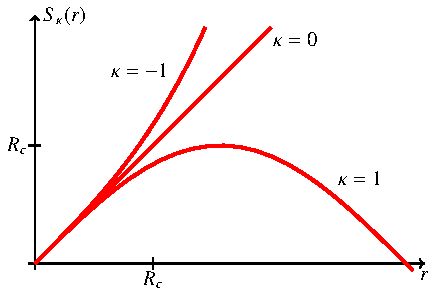
\includegraphics{chapters/tikz/robertson.pdf}
\caption{Darstellung der Funktionen $S_\kappa(r)$ für 
verschiedene Werte von $\kappa$
\label{skript:Skappa:graph}}
\end{figure}

Offenbar spielt für die Lösung  nur das Vorzeichen von $k$ und die
Grösse $R_c$ ein Rolle.
Wir trennen diese beiden Elemente daher, bezeichnen das Vorzeichen
von $k$ mit $\kappa$ und $R_c = 1/\sqrt{2|k|}$.
Wir können $S(r)$ daher auch etwas einheitlicher als
\begin{equation}
S_\kappa(r) = \begin{cases}
R_c\sin  \displaystyle\frac{\mathstrut r}{R_c} &\qquad \kappa= 1\\
r                                              &\qquad \kappa= 0\\
R_c\sinh \displaystyle\frac{\mathstrut r}{R_c} &\qquad \kappa=-1
\end{cases}
\label{skript:rwmetrik:Skappa}
\end{equation}
schreiben.
In Abbildung~\ref{skript:Skappa:graph} sind die Funktionen $S_\kappa(r)$
für $R_c=1$ und für alle drei Werte von $\kappa$ dargestellt.
Ebenfalls erkennbar ist, dass für kleine Werte von $r$ gilt
$S_\kappa(r)\simeq r$.

\subsection{Ableitungen von $S_\kappa(r)$}
Für spätere Verwendung bei der Herleitung der Friedmanngleichungen
in Kapitel~\ref{skript:chapter:friedmann}
berechnen wir die erste und zweite Ableitung 
von $S_\kappa(r)$.
Die erste Ableitung ist
\begin{align*}
S'_\kappa(r)
&=
\begin{cases}
\cos \displaystyle\frac{\mathstrut r}{R_c}&\qquad \kappa= 1\\
1                                         &\qquad \kappa= 0\\
\cosh\displaystyle\frac{\mathstrut r}{R_c}&\qquad \kappa=-1.
\end{cases}
\end{align*}
Wir drücken die rechte Seite des Quadrates hiervon durch $S_\kappa(r)$ aus:
\begin{equation}
S'_\kappa(r)^2
=
\left\{
\begin{aligned}
&\cos^2\displaystyle\frac{\mathstrut r}{R_c}
=
1-\sin^2\displaystyle\frac{\mathstrut r}{R_c}
=
1-\kappa \frac{S_\kappa(r)^2}{R_c^2}&&\qquad\kappa=1\\
&1&&\qquad\kappa=0\\
&\cosh^2\displaystyle\frac{\mathstrut r}{R_c}
=
1+\sinh^2\displaystyle\frac{\mathstrut r}{R_c}
=
1-\kappa \frac{S_\kappa(r)^2}{R_c^2}&&\qquad\kappa=-1.
\end{aligned}
\right.
\end{equation}
Unabhängig von den Werten von $\kappa$ und $R_c$ gilt also immer
\begin{equation}
S'_\kappa(r)^2 = 1-\kappa \frac{S_\kappa(r)^2}{R_c^2}.
\label{skript:robertson:ersteableitung}
\end{equation}
Für die zweite Ableitung finden wir
\begin{align*}
S''_\kappa(r)
&=
\begin{cases}
\displaystyle-\frac{1}{R_c}\sin \frac{\mathstrut r}{R_c}&\qquad \kappa= 1\\
0                                                       &\qquad \kappa= 0\\
\displaystyle \frac{1}{R_c}\sinh\frac{\mathstrut r}{R_c}&\qquad \kappa=-1.
\end{cases}
\end{align*}
Auch dieses Resultat können wir einheitlich als
\begin{equation}
S''_\kappa(r)
=
-\kappa\displaystyle \frac{S_\kappa(r)}{R_c^2}
\label{skript:robertson:zweiteableitung}
\end{equation}
schreiben, was auch aus der Differentialgleichung~\eqref{skript:rwmetrik:Sdgl}
folgt.
Wir fassen die Resultate im folgenden Satz zusammen.

\begin{satz}
\index{skript:satz:isotrope}
Eine homogene und isotrope Metrik eines dreidimensionalen Raumes
hat daher die Form
\begin{equation}
ds^2=dr^2 + S_{\kappa}(r)d\Omega^2.
\label{skript:rwmetrik:metrikS}
\end{equation}
Diese Metrik beschreibt einen Raum mit konstantem
Ricci-Krümmungs\-skalar 
\begin{equation}
R
=
-\frac{S''_\kappa(r)}{S'_\kappa(r)}
=
-\frac{-2\kappa S_\kappa(r)}{S_\kappa(r)R_c^2}
=
\frac{2\kappa}{R_c^2}.
\label{skript:rwmetrik:R}
\end{equation}
\end{satz}
Der Parameter $\kappa$ kann nur die Werte $\pm 1$ und $0$ annehmen, er ist
das Vorzeichen des Ricci-Krümmungs\-skalars \eqref{skript:rwmetrik:R}.
Für $\kappa=1$ ist die Krümmung des Raumes positiv, für $\kappa=-1$ ist
sie negativ, für $\kappa=0$ liegt ein euklidischer Raum vor.
Der Krümmungsradius ist in den Fällen $\kappa=\pm1$ jeweils $R_c$.

\subsection{Der Grenzfall $R_c\to\infty$}
Schreibt man $K_c = 1/R_c$ für die Krümmung, dann kann man $S_0(r)$
auch als Grenzfall von $S_{\pm 1}(r)$ für $K_c\to 0$ erhalten.
Es gilt  nämlich
\begin{equation}
\lim_{R_c\to\infty} S_\kappa(r)
=
\lim_{K_c\to 0} S_\kappa(r)
=\begin{cases}
\displaystyle
\lim_{K_c\to 0}\frac{\displaystyle \sin(K_cr)}{\displaystyle K_c}
=
\lim_{K_c\to 0}\frac{\displaystyle r\cos(K_cr)}{\displaystyle 1} = r = S_0(r)
&\qquad\kappa=1
\\
\\
\displaystyle
\lim_{K_c\to 0}\frac{\displaystyle \sinh(K_cr)}{\displaystyle K_c}
=
\lim_{K_c\to 0}\frac{\displaystyle r\cosh(K_cr)}{\displaystyle 1} = r = S_0(r)
&\qquad\kappa=-1
\end{cases}
\end{equation}
nach der Regel von de l'Hospital.
Die Funktion $S_0(r)$ ist daher der Grenzfall der Funktionen
$S_\kappa(r)$ für unendlich grossen Krümmungsradius $R_c$.

\section{Statisches Universum}
\rhead{Statisches Universum}
\index{statisches Universum}%
Zu Einsteins Zeit gab es keine Hinweise darauf, dass das Universum
sich mit der Zeit verändert.
Es lag daher nahe, nach einer homogenen und isotropen Lösung zu suchen,
die zudem zeitlich unveränderlich ist.
Die Metrik eines solchen Universums muss nach
Satz~\ref{skript:satz:isotrope}
die Form
\[
ds^2
=
-c^2\,dt^2 + dr^2 + S_\kappa(r)^2\,d\Omega^2
\]
haben.
Einzig die der Parameter $\kappa$ und der Krümmungsradius $R_c$ sind
noch wählbar. 
Diese müssen so bestimmt werden, dass ein Universum homogener Dichte
den Einstein-Gleichungen genügt.

Wir bestimmen die $00$-Komponente des Einstein-Tensors mit Hilfe
von Maxima und finden
\begin{align*}
G_{00}
%&=
%-{{2\,c^2\,S\left(r\right)\,\left({{d^2}\over{d\,r^2}}\,S\left(r
% \right)\right)+c^2\,\left({{d}\over{d\,r}}\,S\left(r\right)\right)^2
% -c^2}\over{S^2\left(r\right)}}
%\\
&=
-c^2\frac{ 2S_\kappa(r)S''_\kappa(r) + S'_\kappa(r)^2-1 }{S_\kappa(r)^2}
\end{align*}
Darin können wir die zweite Ableitung durch
\eqref{skript:robertson:zweiteableitung}
ersetzen und das Quadrat der ersten Ableitung durch
\eqref{skript:robertson:ersteableitung}.
Dann wird $G_{00}$ zu
\begin{align*}
G_{00}
&=
-c^2\frac{2\kappa S_\kappa(r)^2/R_c^2 + 1-\kappa S_\kappa(r)^2/R_c^2-1 }{S_\kappa(r)^2}
=
-\frac{c^2\kappa}{R_c^2}
\end{align*}
Setzt man dies in die Einstein-Gleichungen ein, erhalten wir
\begin{equation}
-\frac{c^2\kappa}{R_c^2}=\frac{8\pi K\varrho}{c^2}
\end{equation}
Da die Dichte $\varrho$ positiv ist, liest man daraus ab, dass ein solches
Universum negative Krümmung haben muss.

Man kann jedoch noch einen Schritt weiter gehen und die Spur der
Einstein-Gleichungen berechnen.
Die Verjüngung $G_\mu^\nu$ kann wieder mit Maxima berechnet werden,
sie ist
\begin{align*}
G=G_\mu^\mu
%&=
%{{4\,S\left(r\right)\,\left({{d^2}\over{d\,r^2}}\,S\left(r\right)
% \right)+2\,\left({{d}\over{d\,r}}\,S\left(r\right)\right)^2-2}\over{
% S^2\left(r\right)}}
%\\
&=
2\frac{2S_\kappa(r)S''_\kappa(r) + S'_\kappa(r)^2-1}{S_\kappa(r)^2}
\end{align*}
Die bereits bekannten Ersetzungen
\eqref{skript:robertson:zweiteableitung}
und
\eqref{skript:robertson:ersteableitung}
machen daraus
\begin{align*}
G
&=
2\frac{-2\kappa S_\kappa(r)^2/R_c^2 + 1-\kappa S_\kappa(r)^2/R_c^2-1}{S_\kappa(r)^2}
=
-\frac{6\kappa}{R_c^2}.
\end{align*}
Der Energie-Impuls-Tensor eines idealen Gases hat die Spur
\[
T_\mu^\mu
=
\frac1{c^2}(-\varrho c^2+3p),
\]
damit werden die verjüngten Einstein-Gleichungen zu
\[
G_\mu^\mu
=
-\frac{6\kappa}{R_c^2}
=
\frac{8\pi K}{c^4}(-\varrho c^2 + 3p).
\]
Dividieren wir durch 6 und multiplizieren wir mit $c^2$ erhalten
wir eine weitere Gleichung für $\kappa/R_c^2$.
Insgesamt entsteht so das Gleichungssystem
\begin{align*}
\frac{\kappa c^2}{R_c^2}
&=
\frac{8\pi K\varrho}{c^2}
\\
\frac{\kappa c^2}{R_c^2}
&=
\frac{4\pi K}{3c^2}(-\varrho c^2 + 3p).
\end{align*}
Durch Gleichsetzen bekommen wir eine Bezeihung zwischen Druck und
Dichte.
Diese zweite Gleichung würde also eine Temperatur des Universums 
bereits eindeutig festlegen.
%\begin{align*}
%\frac{8\pi K\varrho}{c^2}
%&=
%\frac{3\pi K}{3c^2}(-\varrho c^2 + 3p)
%\\
%6\varrho
%&=
%-2\varrho+3p
%\end{align*}
Ein mit einem idealen Gas gefülltes statisches Unversum kann also
nur positiv gekrümmt sein und es kann
nur bei einer ganz bestimmten Temperatur existieren.
Da die Sterne Strahlung produzieren
und damit das Universum aufheizen, kann dies keine physikalische
Lösung sein.
Ein statisches Universum ist nicht mit den Einstein-Gleichungen
verträglich.

\section{Expansion des Universums}
\rhead{Expansion des Universums}
Zu Beginn des 20.~Jahrhunderts hatte man noch keine klare Vorstellung
über die Grösse des Universums.
Allgemein wurde angenommen, dass unsere Milchstrasse im wesentlichen das
ganze Universum ist.
Verschiedene neblige Objekte waren seit längerer Zeit bekannt und
katalogisiert worden.
Vor allem Wilhelm Herschel hat in seinem grossen 
\index{Wilhelm Herschel}%
{\em Catalogue of Nebulae and Clusters of Stars} über 2000 Objekte
\index{Catalogue of Nebulae and Clusterse of Stars}%
erfasst.
Diese wurden jedoch meist als Objekte in unserer eigenen Galaxie angesehen.
Auch wurde das Universum im Wesentlichen als unveränderlich angesehen.

In den frühen zwanziger Jahren des 20.~Jahrhunderts gelang es dann
Edwin Hubble, die Entfernung von des {\em Great Andromeda Nebula}
\index{Hubble, Edwin}%
zu bestimmen, wie
die Andromeda Galaxie unter der Nummer 116 in Herschels Katalog verzeichnet
war.
Er verwendete dafür sogenannte Cepheiden-Veränderliche.
Zwischen der absoluten Helligkeit dieser veränderlichen
Sterne und der Periode der Helligkeitsschwankungen besteht
eine einfache Beziehung.
Hubble fand Cepheiden-Veränderliche in Aufnahmen der Andromeda-Galaxie
und war damit in der Lage, deren absolute Helligkeit zu bestimmen.
Aus der beobachteten Helligkeit konnte er die Entfernung ableiten.
Er vermass eine ganze Reihe solcher heller Nebel und konnte so zeigen,
dass sich diese heute als Galaxien erkannten Nebel alle
weit ausserhalb unserer Milchstrasse
befinden.

Hubble und sein Assistent Milton Humason massen mit dem neuen
\index{Humason, Milton}%
2.5m-Hooker-Teleskop neben der Entfernung auch die Spektren und
\index{Hooker-Teleskop}%
damit die Rotverschiebung von 46 Galaxien.
Es zeigte sich, dass sich weiter entfernte Galaxien schneller 
entfernen.
Sie schlossen daraus, dass das Universum expandieren muss, sie konnten
sogar die Geschwindigkeit bestimmen, mit der dies geschieht\footnote{
Später stellte sich heraus, dass die Kalibrierung der Entfernungsskala
etwa um einen Faktor 10 falsch war. Die ersten Kosmologischen Modelle
kamen daher auf ein Alter des Universums, welches kürzer war als das
den Geologen schon längst bekannte Mindestalter der Erde.}.

Der belgische Physiker
Georges Lemaître hatte auf der Basis von Einsteins allgemeiner
\index{Lemaître, Georges}%
Relativitätstheorie die Expansion des Universums bereits vor
Hubbles Entdeckung vorhergesagt.
Doch erst die Messungen von Hubble und Humason haben bewiesen,
dass Einsteins Theorie die Entwicklung des Universums korrekt
vorhersagen kann.

\subsection{Der Skalenfaktor}
\begin{figure}
\centering
\includegraphics[width=\hsize]{chapters/tikz/expansion1.pdf}
\caption{Expansion des Universums um einen Beobachter im ``Zentrum''
\label{skript:figure:expansion1}}
\end{figure}
\begin{figure}
\centering
\includegraphics[width=\hsize]{chapters/tikz/expansion2.pdf}
\caption{Expansion des Universums. Da sich das Univerum überall
mit dem gleichen Skalenfaktor ausdehnt, erscheinen sich für jeden
Beobachter die Galaxien mit der gleichen Geschwindigkeit zu entfernen.
Die Fluchgeschwindigkeit ist kein Hinweis darauf, dass im Universum
einen bevorzugten Punkt gäbe (Homogenität).
\label{skript:figure:expansion2}}
\end{figure}
Hubbles Beobachtungen haben gezeigt, dass sich das Universum ausdehnt.
Zwei nahe Punkte befinden sich zur Zeit $t_0$ in einem Abstand $d_0$,
und sollen in einem geeigneten Koordinatensystem in Ruhe sein.
Zu einer späteren Zeit wird die Distanz sich vergrössert haben.
Da das Universum isotrop und homogen ist, muss die Distanz in jeder
beliebigen Richtung um den gleichen Faktor gewachsen sein.
Die Ausdehnung des Universums ist also eine Ähnlichkeitstransformation.
Sie kann durch eine einzige, von der Zeit abhängige Zahl,
den {\em Skalenfaktor} $a(t)$ beschrieben werden.
\index{Skalenfaktor}%
Wir geben der Funktion $a(t)$ willkürlich den Wert $1$ für die heutige
Zeit, die wir im Folgenden mit $t_0$ bezeichnen.

Die Tatsache, dass ein Beobachter alle Galaxien sich entfernen
sieht, bedeutet nicht, dass das Universum ein Zentrum hat.
Auch für jeden anderen Beobachter werden die Distanzen zu den
Galaxien grösser und zwar um den gleichen Faktor
(Abbildungen~\ref{skript:figure:expansion1} und
\ref{skript:figure:expansion2}).

\subsection{Die Hubble-Konstante und das Alter des Universums}
\index{Hubble-Konstante}%
\index{Alter des Universums}%
Nehmen wir an, dass das Universum sich mit konstanter Geschwindigkeit
ausdehnt, dass also 
\[
H(t)=H_0=\frac{\dot a(t)}{a(t)}
\]
gilt.
\index{Hubble-Konstante}%
Dies ist eine Differentialgleichung für $a(t)$, die wir sofort
lösen können:
\[
a(t) = H_0a(t)
\qquad \Rightarrow\qquad
a(t)=H_0 e^{t-t_0}.
\]
Wir erhalten daher einen exponentiell anwachsenden Skalenfaktor,
wofür es keinen experimentellen Hinweis gibt und der auch physikalisch
unsinnig scheint.
$H(t)$ kann also keine Konstante sein.

Nehmen wir aber an, dass $\dot a(t)$ konstant ist, dann ist $a(t)$
eine lineare Funktion der Zeit mit Steigung  $H_0$ zur Zeit $t=t_0$,
also
\[
a(t)=H_0(t-t_0) + 1.
\]
Daraus können wir den Zeitpunkt berechnen, zu dem der Skalenfaktor
$a(t)=0$ war, es muss
\[
t-t_0 = -\frac1{H_0}
\]
gelten.
Man nennt $1/H_0$ die {\em Hubble-Zeit}.
\index{Hubble-Zeit}%
Der beste bekannte Wert für $H_0$ wurde mit der Planck-Mission als
\index{Planck-Mission}%
\begin{equation}
H_0
=
(67.74 \pm 0.46)\frac{\text{km}}{\text{s}\cdot\text{Mpc}}
=
(2.1951\pm 0.0149)
10^{-18}\frac{1}{\text{s}}
\label{skript:robertson:hubble0}
\end{equation}
bestimmt.
Die zugehörige Hubble-Zeit ist
\begin{equation}
\frac{1}{H_0} = 14.4\text{Gyr}.
\label{skript:robertson:hubblezeit}
\end{equation}
Wenn wir annehmen, dass die im Universum enthaltene Masse die Ausdehnung
verlangsamt, muss die Hubble-Zeit eine obere Schranke für das Alter
des Universums sein.

\subsection{Hubble-Distanz%
\label{skript:section:hubble-distanz}}
\index{Hubble-Distanz}%
Zwei Punkte, die sich zur Zeit $t$ im Abstand $l$ befinden, entfernen
sich voneinander mit der Geschwindigkeit $Hl$. 
Da sich nichts schneller als mit Lichtgeschwindigkeit durch die
Raumzeit bewegen kann, ist jede Einflussnahme zwischen diesen zwei
Punkten unmöglich, wenn $Hl>c$ ist.
Folglich sind Punkt gegenseitig unerreichbar, wenn ihre Distanz
\begin{equation}
l > \frac{c}{H}
\label{skript:robertson:hubbledistanz}
\end{equation}
ist.
Die Distanz $c/H$ heist die {\em Hubble-Distanz}.
\index{Hubble-Distanz}%
Wieder aus aktuellen Zahlenwerten für $c$ und $H_0$ finden wird
\[
\frac{c}{H_0}
=
\frac{2.99792458\cdot 10^{8}}{2.1951\cdot 10^{-18}}
=
1.3657\cdot 10^{26}\,\text{m}
\simeq
14.4\,\text{Lichtjahre}
\]
als aktuelle Hubble-Distanz.

\section{Robertson-Walker-Metrik}
%\rhead{Robertson-Walker-Metrik}
Das Universum ist auf grosse Distanzen homogen und isotrop.
Die Einstein-Gleichungen müssen daher auch eine Metrik als
Lösung zulassen, die homogen und isotrop ist.
Bis jetzt haben nur Metriken für den dreidimensionalen Raum
studiert.
In diesem Abschnitt wollen wir untersuchen, wie die Metrik einer
homogenen und isotropen vierdimensionalen Raumzeit
beschaffen sein muss.

\rhead{Robertson-Walker-Metrik}

\subsection{Metrik}
Wenn kein Standort im Universum bevorzugt ist, dann muss es
eine universelle Zeitkoordinaten $t$ geben, die Metrik muss
sich schreiben lassen in der Form
\[
ds^2
=
-c^2\,dt^2
+
g_{ij}\,dx^i\,dx^j,
\]
wobei wie früher lateinische Indizes andeuten sollen, dass die
Summation nur über die Raumkoordinaten zu erstrecken ist.
Wäre dies nicht möglich, dann müsste der Koeffizient von $dt^2$
in einem Raumpunkt von $-c^2$ abweichen.
Dieser Punkt hätte dann aber andere Eigenschaften als alle anderen
Punkte im Universum, was das kosmologische Prinzip verletzt.

Da wir jetzt die Zeitabhängigkeit wie auch die Ortsabhängigkeit der
Metrik eines isotropen und homogen gekrümmten Raumes bereits aus
\eqref{skript:rwmetrik:metrikS} kennen, können
wir die allgemeinste Form der vierdimensionalen Metrik eines solchen
Raumes angeben.

\begin{satz}
Ein homogenes, isotropes Universum hat eine Metrik der Form
\begin{equation}
ds^2
=
-c^2 dt^2 + a(t)^2\bigl(
dr^2 + S_\kappa(r)^2(d\vartheta^2 + \sin^2\vartheta\, d\varphi^2)
\bigr)
=
-c^2 dt^2 + a(t)^2\bigl(
dr^2 + S_\kappa(r)^2 d\Omega^2
\bigr)
\label{skript:rwmetrik:metrik}
\end{equation}
mit $\kappa\in\{0,\pm1\}$ und 
$S_\kappa(r)$ ist eine der Funktionen
\[
S_\kappa(r)
=
\begin{cases}
R_c\sin \displaystyle\frac{\mathstrut r}{R_c}&\qquad \kappa= 1\\
r&\qquad \kappa=0\\
R_c\sinh\displaystyle\frac{\mathstrut r}{R_c}&\qquad \kappa=-1.
\end{cases}
\]
\end{satz}
Die Metrik \eqref{skript:rwmetrik:metrik} heisst die
{\em Robertson-Walker-Metrik}.

\subsection{Geodäten}
Wir bestimmen die Geodätengleichungen in der Robertson-Walker Metrik.
Die allgemeine Geodätengleichung hat die Form
\[
\frac{d^2x^\mu}{ds^2} = -\Gamma^\mu_{\alpha\beta} \dot x^\alpha \dot x^\beta.
\]
Man muss also als Erstes die Christoffelsymbole bestimmen.  
Diese sind auch deshalb interessant, weil $\Gamma^0_{kk}$ in erster
Näherung die Gravitationskräfte beschreibt.

Für jeden Index $\mu$ bilden die $\Gamma^\mu_{\alpha\beta}$
eine symmetrische Matrix.
Für $\mu=0$ zum Beispiel finden wir
\begin{align*}
\Gamma^0_{\alpha\beta}
&=
\begin{pmatrix}
%(%i5) 		        ratsimp(Christoffel2(1, 1, 1))
%(%o5) 				       0
%(%i6) 		        ratsimp(Christoffel2(1, 1, 2))
%(%o6) 				       0
%(%i7) 		        ratsimp(Christoffel2(1, 1, 3))
%(%o7) 				       0
%(%i8) 		        ratsimp(Christoffel2(1, 1, 4))
%(%o8) 				       0
0&0&0&0\\
%(%i9) 		        ratsimp(Christoffel2(1, 2, 2))
%				     d
%			       a(t) (-- (a(t)))
%				     dt
%(%o9) 			       ----------------
%				       2
%				      c
%(%i10) 		        ratsimp(Christoffel2(1, 2, 3))
%(%o10) 				       0
%(%i11) 		        ratsimp(Christoffel2(1, 2, 4))
%(%o11) 				       0
0&\frac1{c^2} a(t)\dot a(t)& 0 & 0 \\
%(%i12) 		        ratsimp(Christoffel2(1, 3, 3))
%			     2	        d
%			    S (r) a(t) (-- (a(t)))
%					dt
%(%o12) 			    ----------------------
%				       2
%				      c
%(%i13) 		        ratsimp(Christoffel2(1, 3, 4))
%(%o13) 				       0
0 & 0 & \frac1{c^2}a(t)\dot a(t)S_\kappa(r)^2 & 0 \\
%(%i14) 		        ratsimp(Christoffel2(1, 4, 4))
%		       2	  d	        2
%		      S (r) a(t) (-- (a(t))) sin (theta)
%				  dt
%(%o14) 		      ----------------------------------
%				       2
%				      c
0 & 0 & 0 & \frac1{c^2} a(t)\dot a(t)S_\kappa(r)^2 \sin^2\vartheta
\end{pmatrix}
\\
&=
\frac1{c^2}
\frac{\dot a(t)}{a(t)}
\begin{pmatrix}
0&     0&                  0&                                 0\\
0&a(t)^2&                  0&                                 0\\
0&     0&a(t)^2S_\kappa(r)^2&                                 0\\
0&     0&                  0&a(t)^2S_\kappa(r)^2\sin^2\vartheta
\end{pmatrix}.
\end{align*}
Die Matrix in der letzten Zeile stimmt bis auf die $00$-Komponente
mit der Metrik überein.
Der Faktor $\dot a(t)/a(t)$ beschreibt die Ausdehungsgeschwindigkeit
des Universums.
Insbesondere sind Strahlen mit
$\vartheta=\operatorname{const}$
und
$\varphi=\operatorname{const}$
Geodäten.

%\subsection{Die Ausdehnung des Universums}
%Aus Metrik eines homogenen und isotropen Raumes gemäss
%\eqref{skript:rwmetrik:metrikS}
%können wir jetzt die allgemeine Metrik einer homogenen und
%isotropen Raumzeit konstruieren.
%Die Metrik
%\begin{equation}
%ds^2
%=
%-c^2\,dt^2 
%+
%a(t)^2\bigl( dr^2 + S_\kappa(r) \,d\Omega^2\bigr)
%\label{skript:rwmetrik:rwmetrik}
%\end{equation}
%heisst die Robertson-Walker-Metrik.
%Wir können sie verwenden, um die Entwicklung des Universums zu
%modellieren.

\section{Wie ist das Universum gekrümmt?}
\rhead{Wie ist das Universum gekrümmt?}
\begin{figure}
\centering
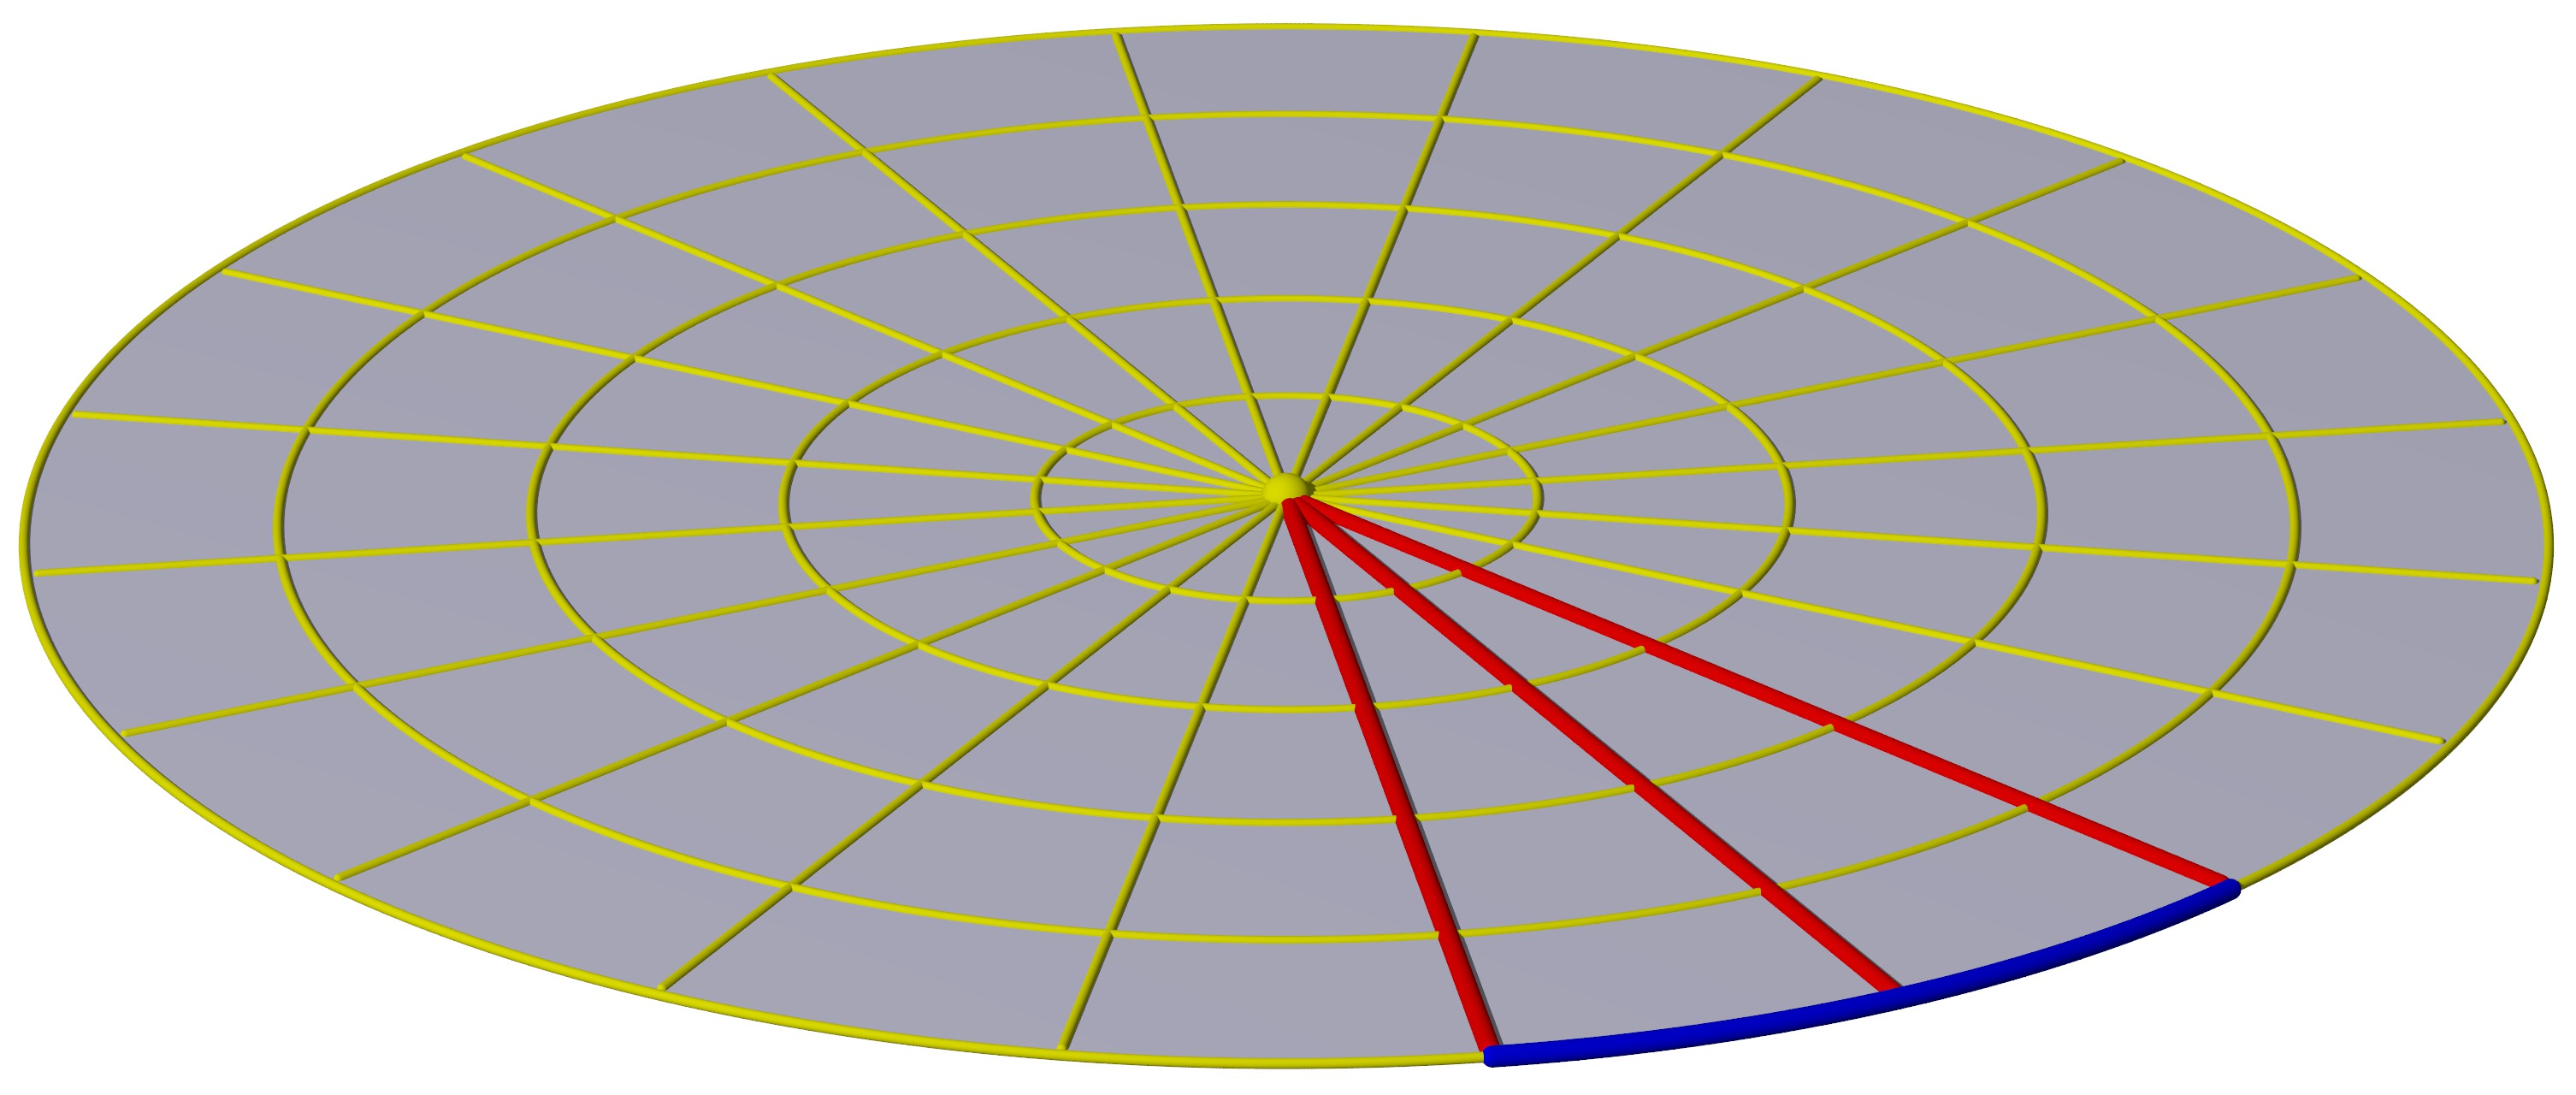
\includegraphics[width=0.7\hsize]{chapters/3d/pringles-flach.jpg}
\caption{Zwei Strahlen (rot), die im Nullpunkt den Winkel $\alpha$
einschliessen, spannen im Abstand $r$ vom Ursprung die Strecke
$\alpha r$ (blau) ein.
\label{skript:pringles:flach}}
\end{figure}
%
\begin{figure}
\centering
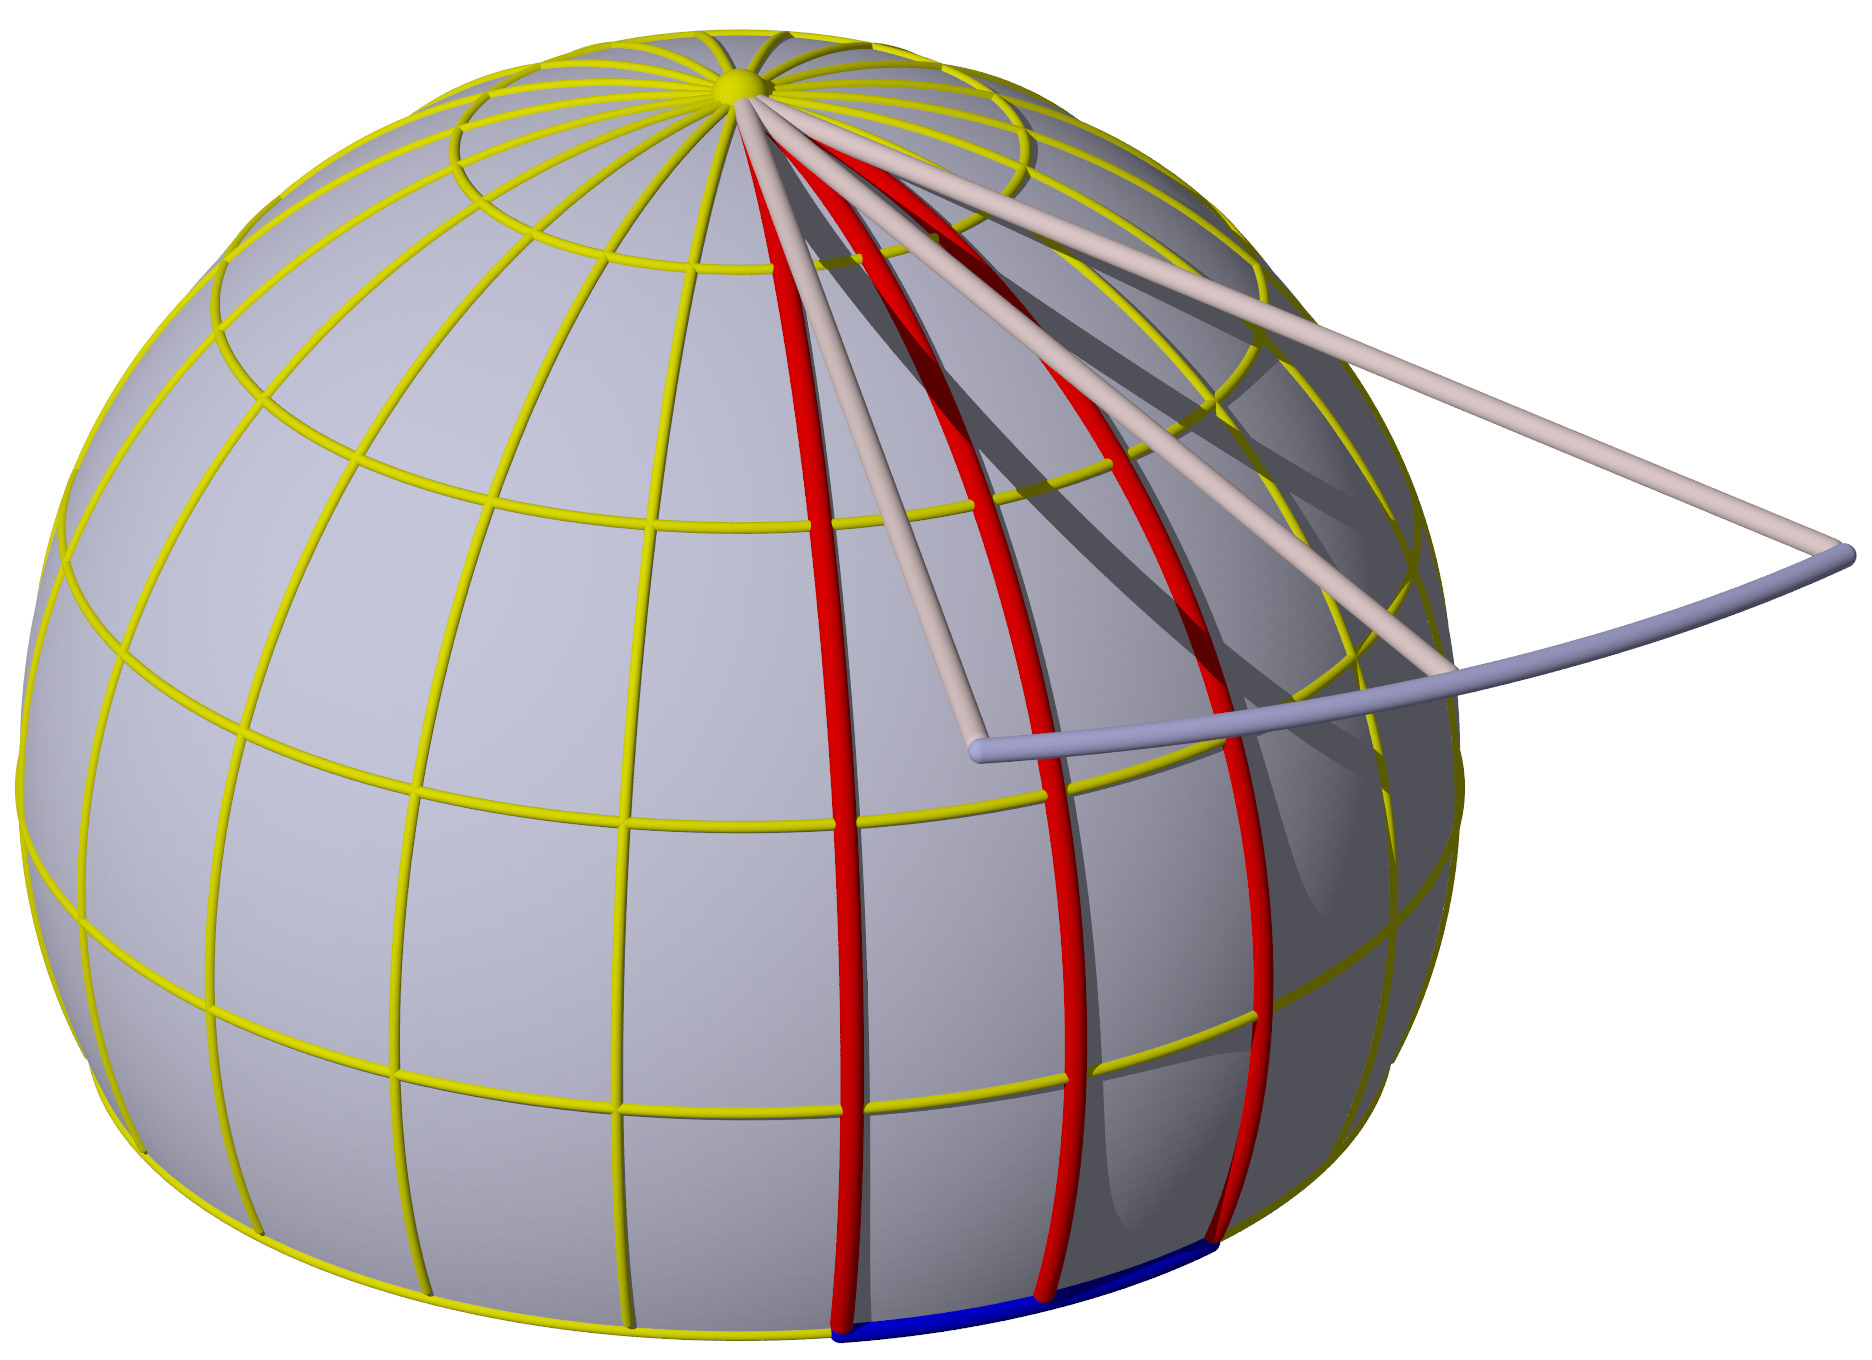
\includegraphics[width=0.7\hsize]{chapters/3d/pringles-positiv.jpg}
\caption{Zwei Geodäten (rot) auf einer positiv gekrümmten Fläche,
die im Nullpunkt den Winkel $\alpha$ einschliessen, spannen im Abstand
$r$ vom Ursprung die Strecke (blau) ein, die kleiner ist als
$\alpha r$.
\label{skript:pringles:positiv}}
\end{figure}
%
\begin{figure}
\centering
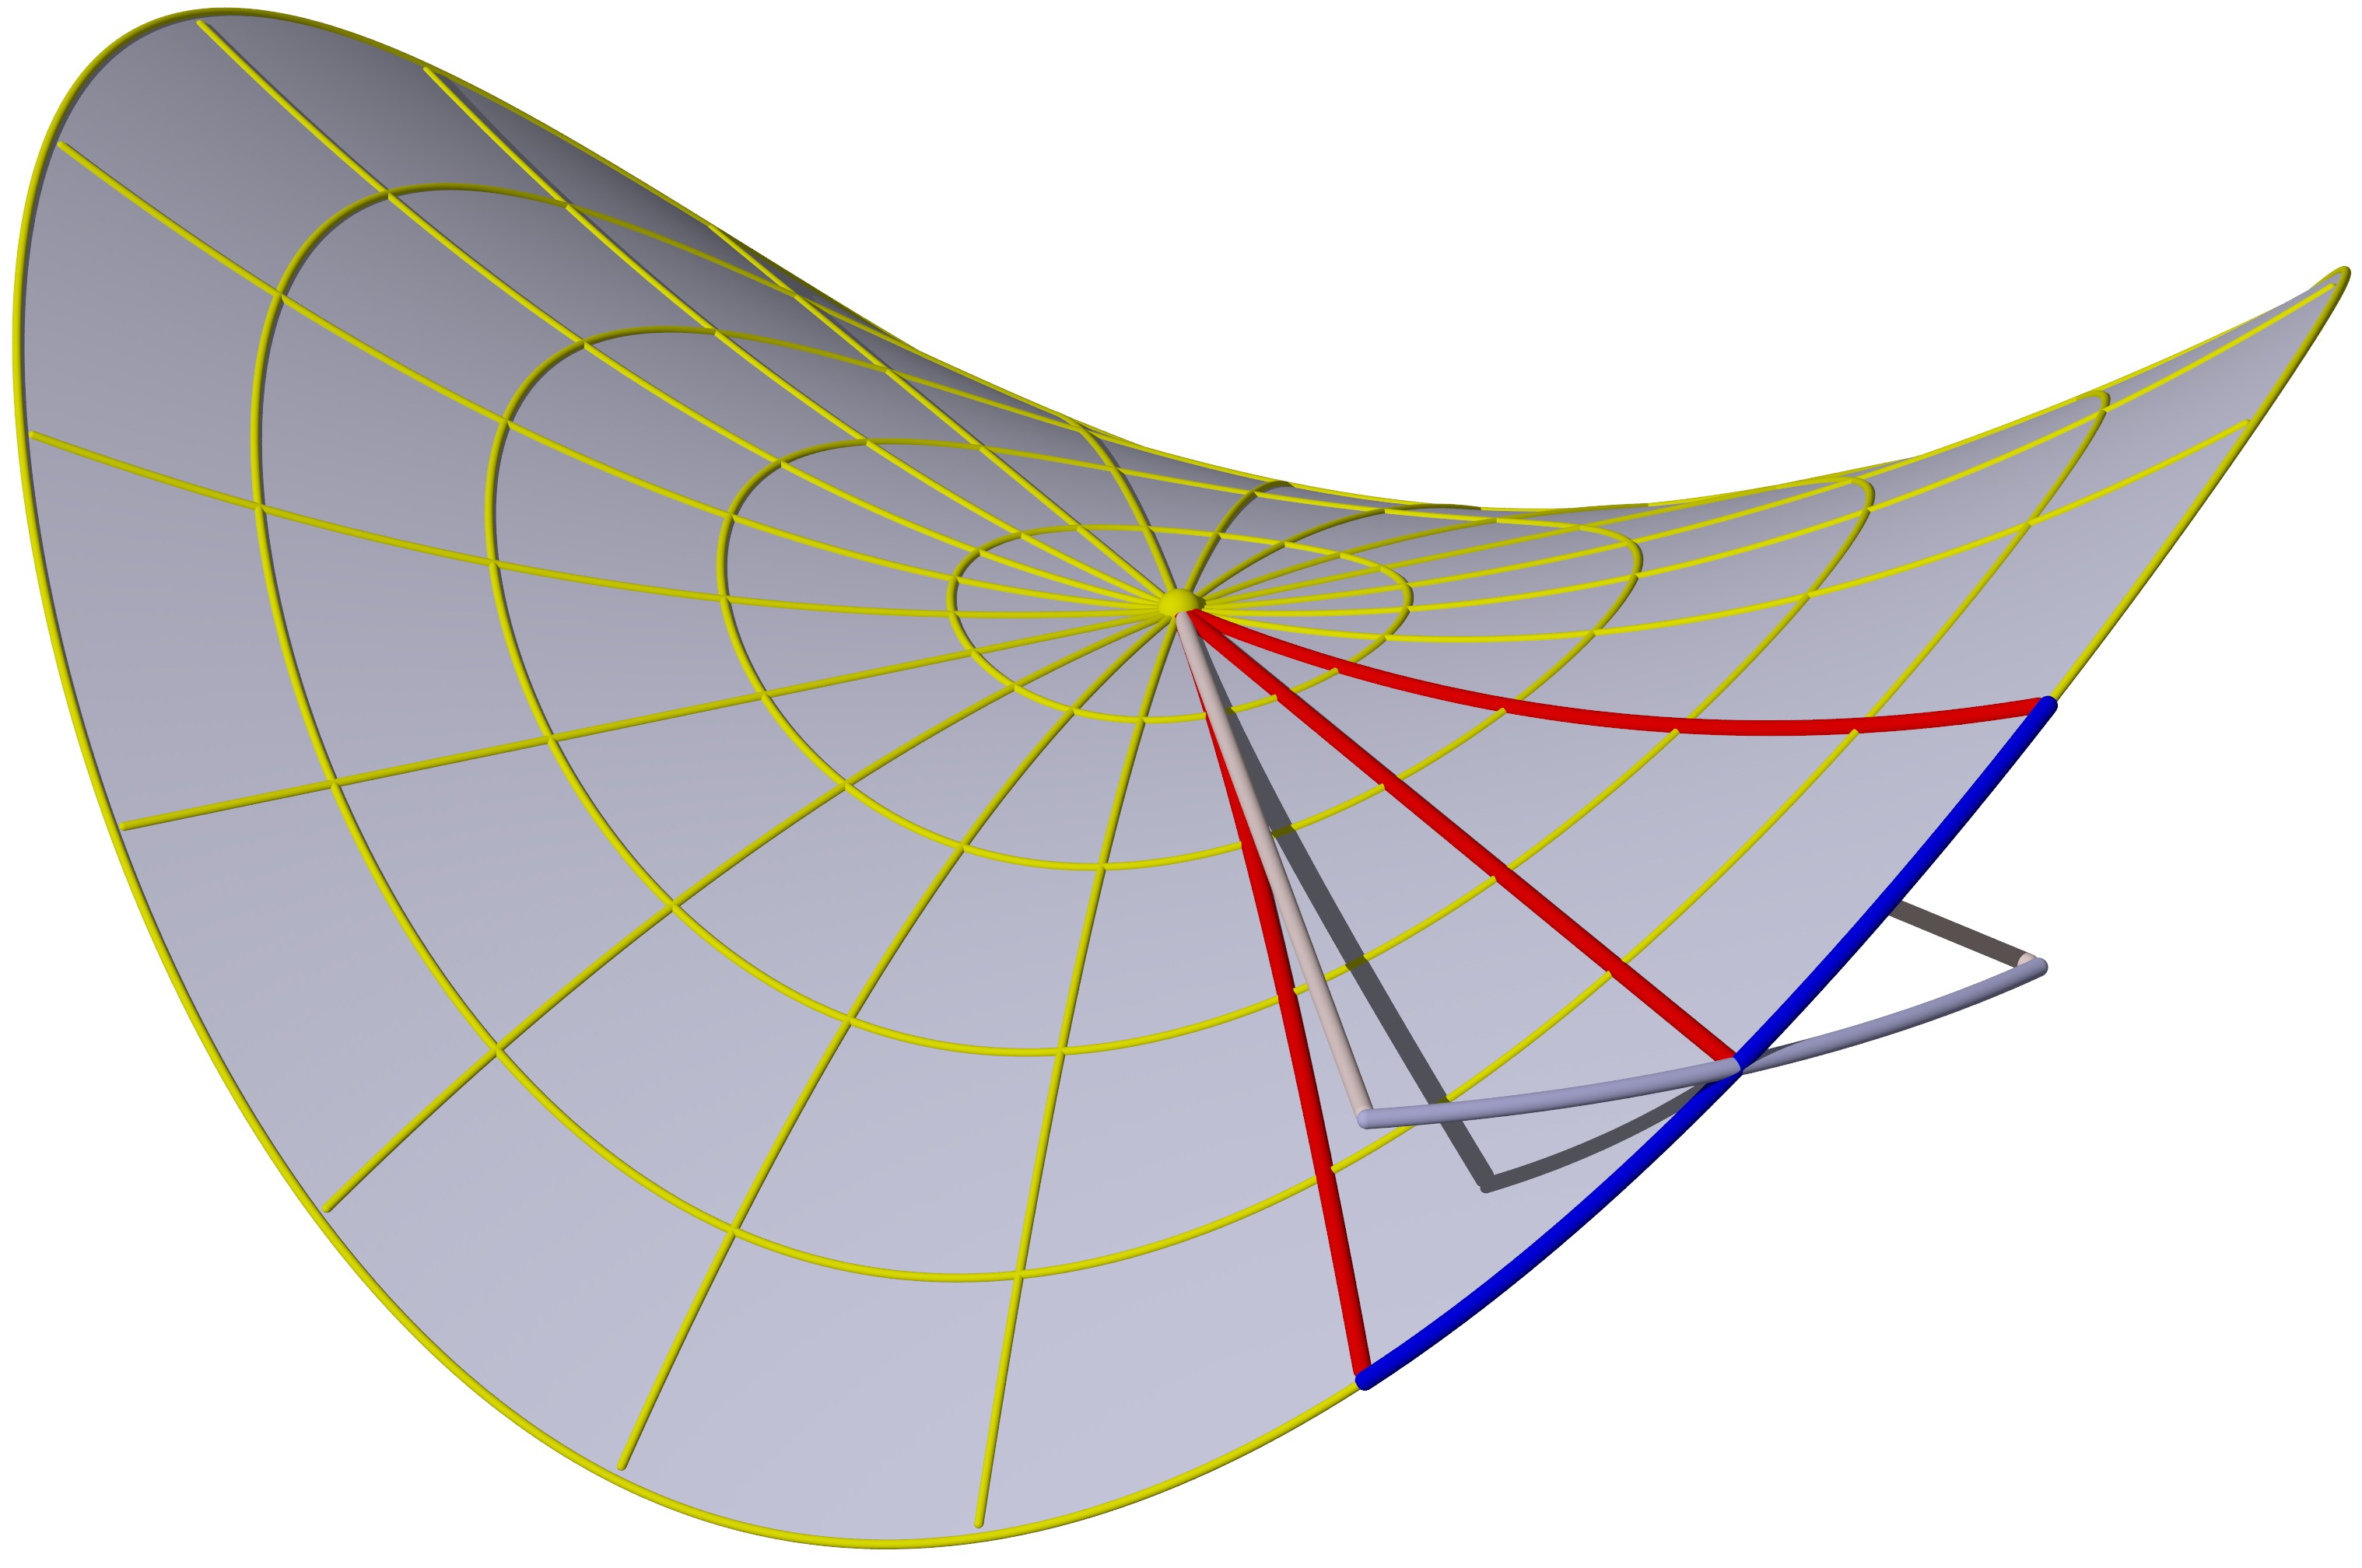
\includegraphics[width=0.9\hsize]{chapters/3d/pringles-negativ.jpg}
\caption{Zwei Geodäten (rot) auf einer negativ gekrümmten Fläche,
die im Nullpunkt den Winkel $\alpha$ einschliessen, spannen im Abstand
$r$ vom Ursprung die Strecke (blau) ein, die grösser ist als
$\alpha r$.
\label{skript:pringles:negativ}}
\end{figure}
%
\begin{figure}
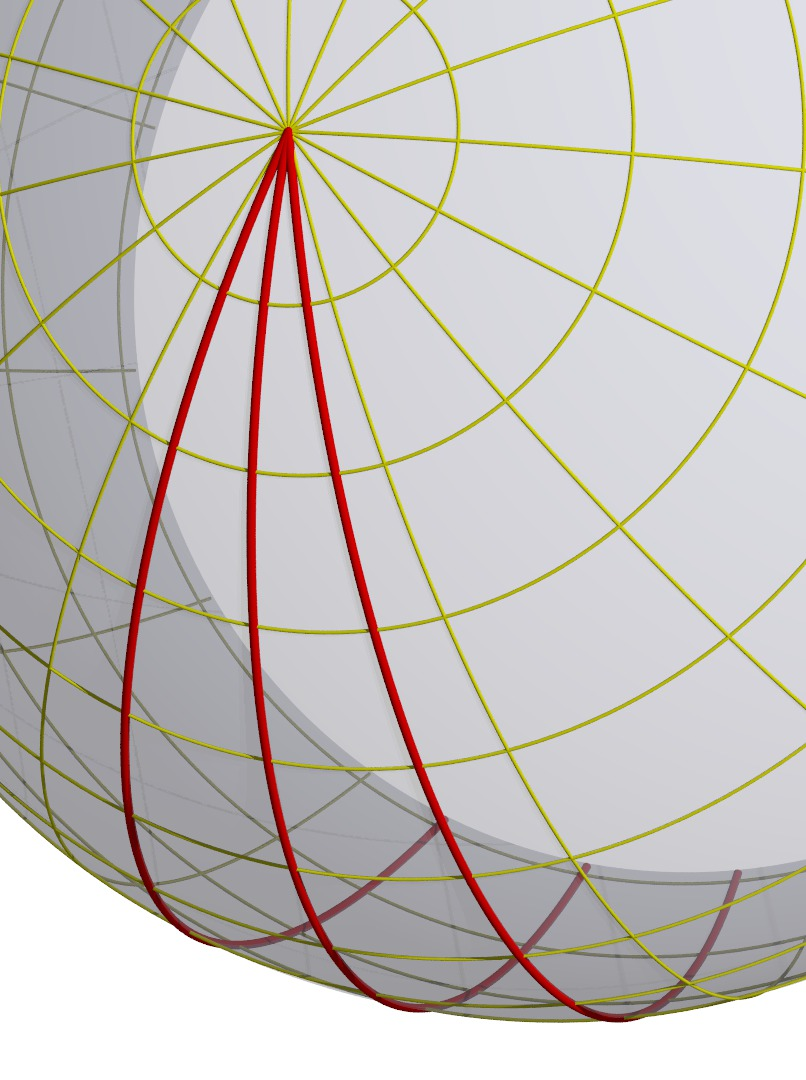
\includegraphics[height=6truecm]{chapters/3d/positiv.jpg}
\quad
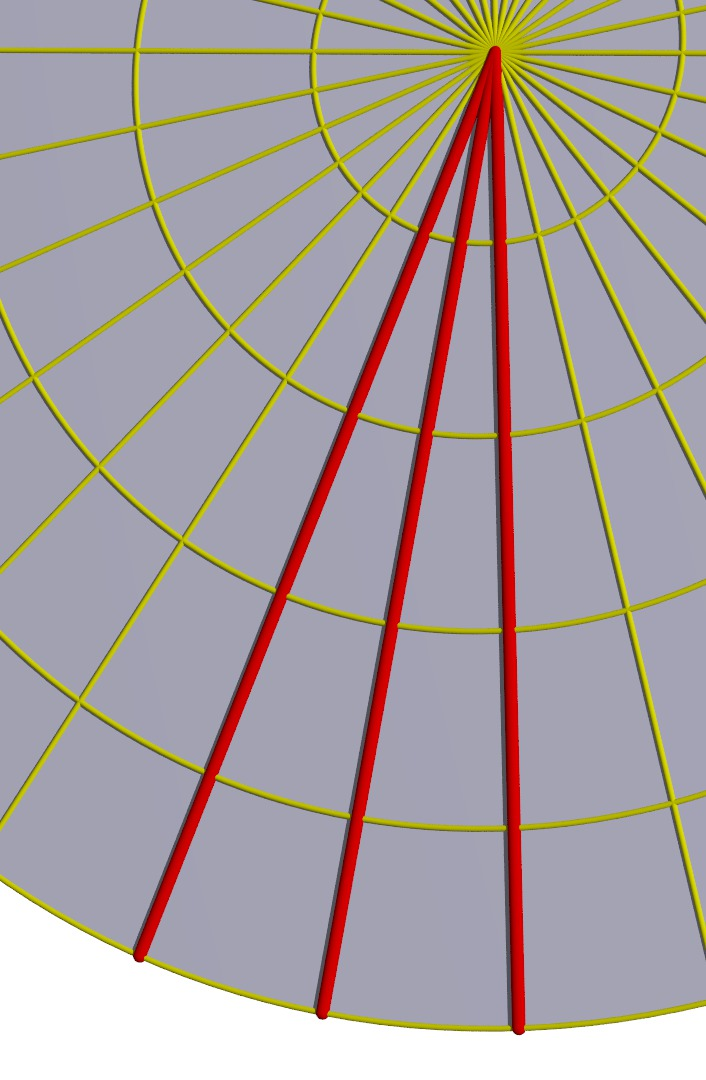
\includegraphics[height=6truecm]{chapters/3d/eben.jpg}
\quad
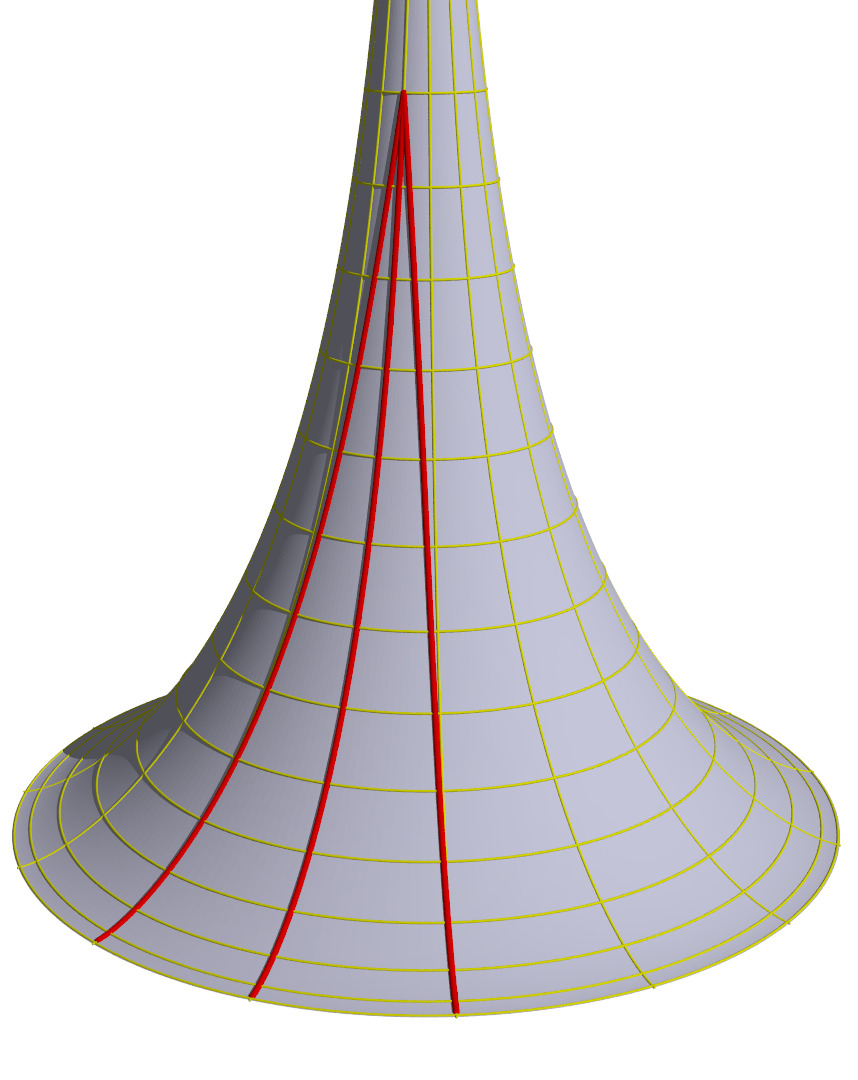
\includegraphics[height=6truecm]{chapters/3d/negativ.jpg}
\caption{Gleichschenklige Dreiecke mit gleichen Seitenlängen in einem
Universum mit positiver Krümmung (links), einem flachen Universum (Mitte)
und einem Universum mit negativer Krümmung (rechts).
Bei einem Universum mit positiver Krümmung ist der Winkel gegenüber
der kurzen Seite grösser als beim flachen Universum, bei einem
Universum mit negativer Krümmung ist er kleiner.
\label{skript:robertson:vergroesserung}}
\end{figure}
Nachdem wir jetzt verstanden haben, wie die Metrik aussehen muss,
bleiben die Parameter $\kappa$, $R_c$ und die Funktion $a(t)$
zu bestimmen.
Dazu werden wir die Einstein-Gleichungen im
Kapitel~\ref{skript:chapter:friedmann} lösen müssen.
Wir werden dabei insbesondere sehen, dass das Universum aus einem
heissen und dichten Anfangszustand entstanden sein muss, dem Big Bang.

Der Parameter $\kappa$ hat besonders drastische
Auswirkungen auf die Geometrie.
Ob das Universum positiv oder negativ gekrümmt oder gar flach ist,
muss experimentell bestimmt werden.
Dazu kann man den Winkel eines gleichschenkligen Dreiecks mit den
Seiten $l$ und $L$ mit $L\gg l$ verwenden.
In einem flachen Universum ist der Winkel gegenüber der Seite $l$
in Bogenmass $l/L$.
In einem Universum mit positiver Krümmung wird ein grösserer Winkel
beobachtet, in einem Universum mit negativer Krümmung ist der Winkel
dagegen kleiner.
Die Abbildung~\ref{skript:robertson:vergroesserung} veranschaulicht
diese vergrössernde Wirkung eines positiv gekrümmten Universums
und die verkleinernde Wirkung eines negativ gekrümmten Universums.

Um zu entscheiden, welchen Wert $\kappa$ für unser Universum hat,
kann man ein Dreieck verwenden, welches als $L$ die Entfernung zum kosmischen
Mikrowellenhintergrund verwendet.
Als kurze Seite des Dreiecks muss eine bekannte Grösse auf der
Fläche der letzten Streuung verwendet werden, von der der der
Mikrowellenhintergrund ausgestrahlt wurde.
Für diesen Zweck zur Verfügung stehen Fluktuationen im kosmischen
Mikrowellenhintergrund.
\index{kosmischer Mikrowellenhintergrund}%
\index{CMB}%
\index{cosmic microwave background}%
Man muss also die Entstehung und vor allem die Abmessungen solcher
Fluktuationen verstehen und berechnen können, bevor man den Test
durchführen kann.
Dies wird im Kapitel \ref{skript:chapter:cmb} durchgeführt, weitere
Informationen zur Analyse des kosmischen Mikrowellenhintergrundes
mit Hilfe von Kugelfunktionen findet man auch im Kapitel~\ref{chapter:cmb}.

\section{Steady State Universum}
\rhead{Steady State Universum}
Die Schlussfolgerung, dass das Universum vor relativ kurzer Zeit
aus einem heissen, dichten 
Zustand hervorgegangen sein müsse, war nicht von Anfang an akzeptiert.
Als alternative Hypothese wurde vorgeschlagen, dass das Universum 
zwar expandiert, dass es dies aber schon seit ewigen Zeiten tut, und dass die
enstehenden
Lücken zwischen den Galaxien dadurch gefüllt werden, dass ständig
neue Materie entstand.
Dazu müsste pro Kubikkilometer und Jahr ein neues Wasserstoffatom
entstehen.
Fred Hoyle
\index{Hoyle, Fred}%
war ein lautstarker Beführworter dieser sogentannten
Steady-State-Hypothese.
\index{Steady-State-Universum}%

Die Steady-State-Hypothese widerspricht jedoch zwei
im Folgenden diskutierten Beobachtungen.

\subsection{Das Paradoxon von Olbers}
\begin{figure}
\centering
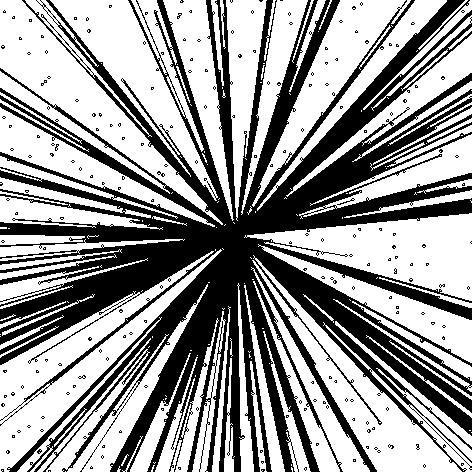
\includegraphics[width=\hsize]{chapters/tikz/wald.pdf}
\caption{Olbers-Paradoxon: Wäre das Universum unendlich ausgedehnt,
sähe man in jeder Richtung irgend wann einen Stern, so dass der Himmel
hell wie die Sonnenoberfläche erscheinen müsste.
\label{skript:figure:waldolbers}}
\end{figure}
\begin{figure}
\centering
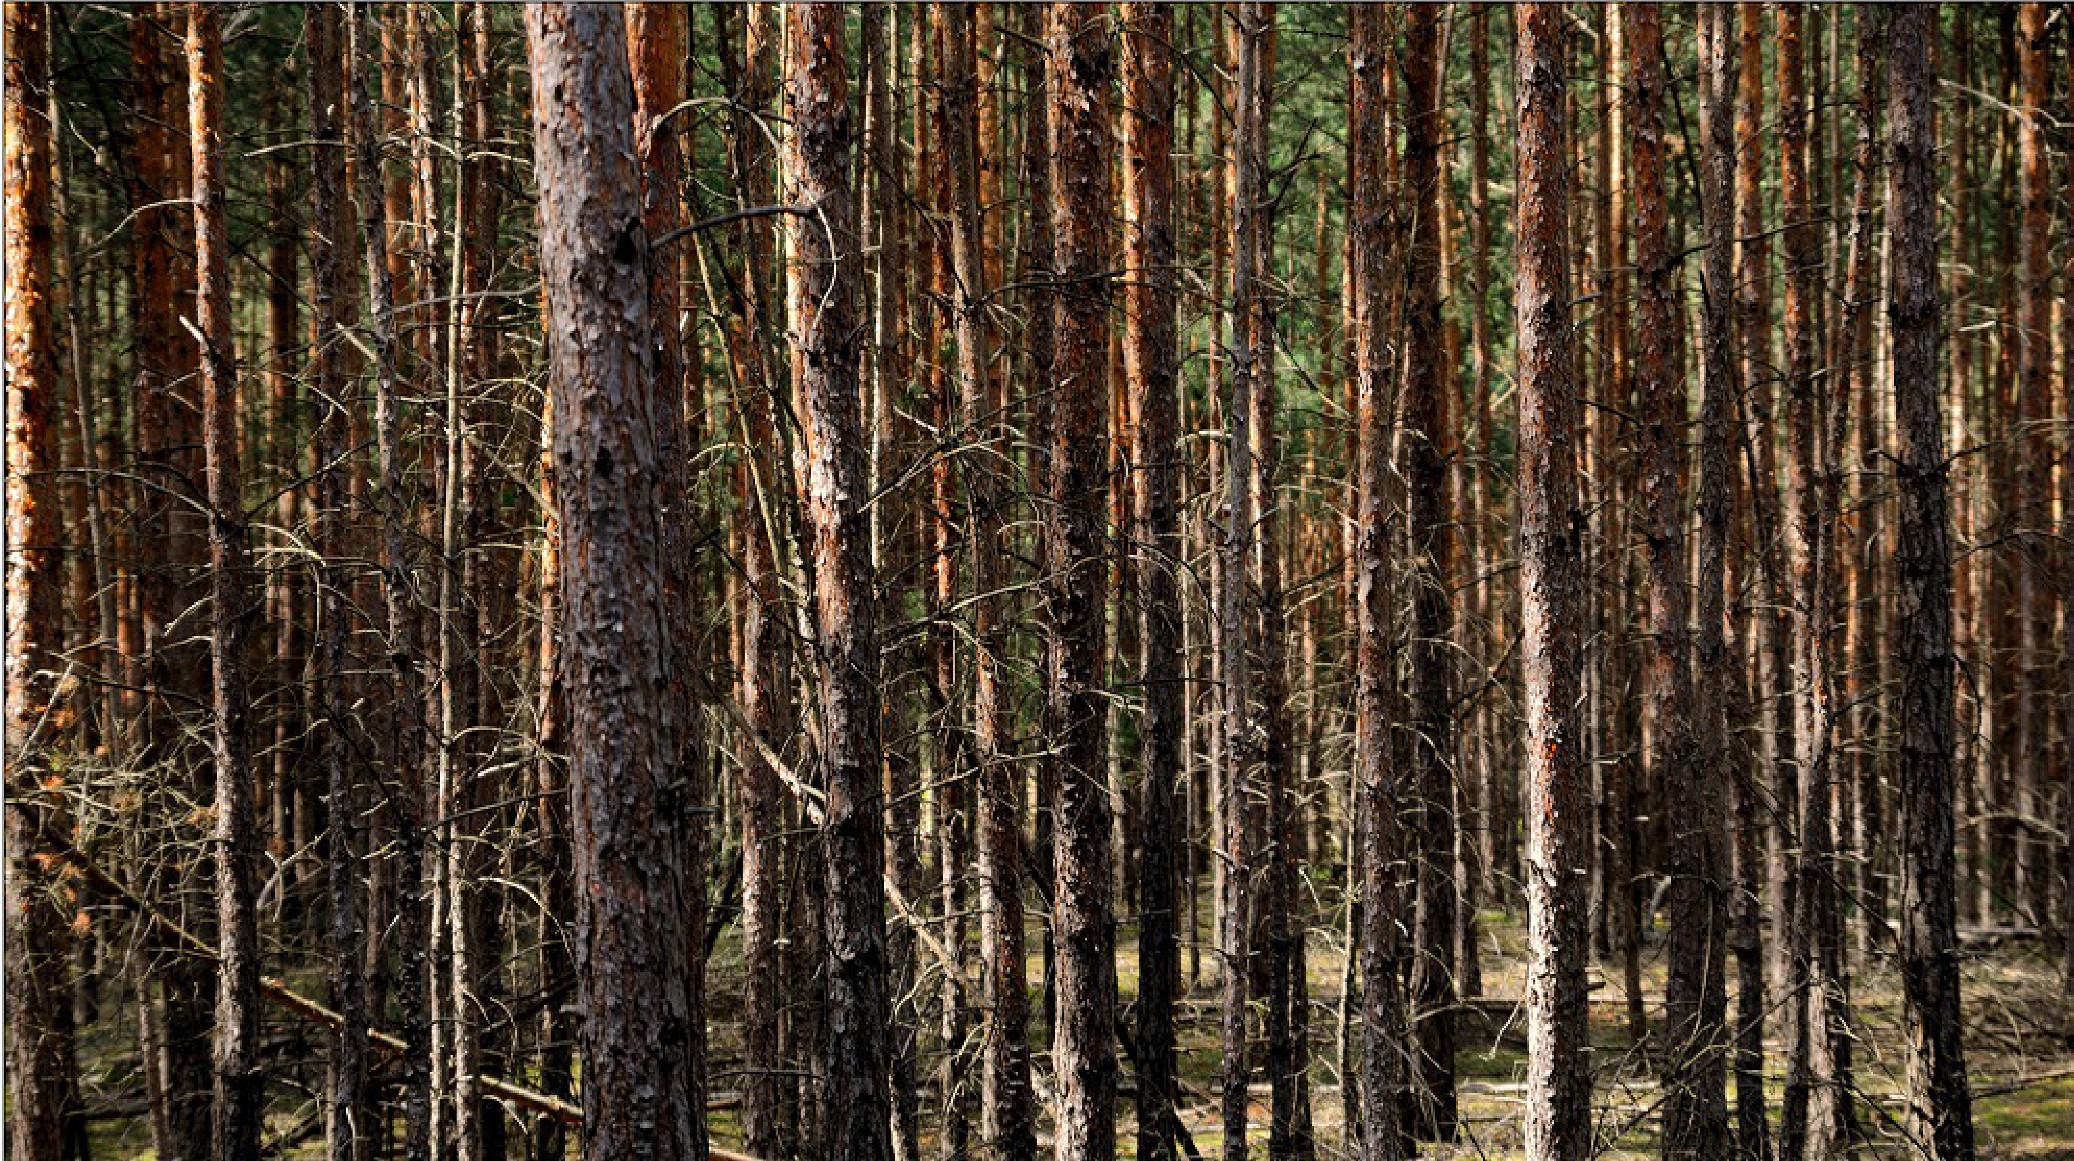
\includegraphics[width=\hsize]{chapters/images/wald50.jpg}
\caption{In einem grossen Wald sieht man in jeder Richtung irgendwann
nur einen Baumstamm, man kann also nicht aus dem Wald heraussehen.
Dies illustriert das Olbers-Paradoxon
\label{skript:robertson:olberswald}}
\end{figure}
In einem grossen Wald (Abbildung~\ref{skript:robertson:olberswald})
trift der Blick in jeder Richtung irgendwann auf einen Baumstamm.
Wenn das Universum unendlich alt und gross ist, dann wird man
man in jeder beliebigen Richtung nicht beliebig weit sehen können,
sondern wie beim Wald wird der Blick irgendwann auf einen Stern treffen.
Der ganze Himmel müsste daher die Helligkeit von Sternen haben.

Nimmt man dagegen an, dass das Universum relativ jung ist, dann kann
man wegen der Endlichkeit der Lichtgeschwindigkeit nur soweit sehen,
wie das Alter des Universums erlaubt.
Das Olbers-Paradox verbietet also nur ein unendlich grosses, homogenes
Universum, in dem man beliebig weit sehen kann. 
Ein junges Universum erfüllt diese Voraussetzung nicht. 
Es könnte aber auch sein, dass Staub den Blick versperrt, so dass selbst
ein unendlich grosses und altes Universum nicht den Beobachtungen entspricht.
Infrarotstrahlung wird jedoch weit weniger vom Staub blockiert, so dass
mindestens im Infrarotlicht der Himmel immer noch strahlend hell sein
müsste.
Neuere Beobachtungen zeigen ausserdem, dass die Menge an Staub im
Universum viel zu gering ist, um den weissen Hintergrund des
Olbers-Paradoxons zu verhindern.

\subsection{Der kosmische Mikrowellenhintergrund}
Im Jahre 1964 entdeckten Penzias und Wilson die kosmische
\index{Penzias, Arno}%
\index{Wilson, Robert Woodrow}%
Mikrowellenhintergrundstrahlung (Siehe auch Kapitel~\ref{chapter:cmb}).
Das Steady-State Modell kann diese isotrope Strahlung nicht erklären.
Das Big-Bang-Modell sagt dagegen einen Strahlungshintergrund mit einem
Schwarzkörperspektrum zu genau der Temperatur voraus, die gemessen
wurde.




